% if you want to print your thesis on one side on the papar, use 'oneside' option 
% if you want to print your thesis on both sides on the papr, do not use 'oneside' option
% the template will generate blank pages bwteen title pages, sections, list of contents ...
\documentclass[11pt,b5paper,oneside]{snuthesis-kor}
%\documentclass[11pt,b5paper]{snuthesis-kor}
%\special{papersize=8.5in,11in}

%%%%%%%%%%%%%%%%%%%%%%%%%%%%%%%%%%%%%%%%%%%%%%%
% include additional packages you need to use
%%%%%%%%%%%%%%%%%%%%%%%%%%%%%%%%%%%%%%%%%%%%%%%
% graphic, float package
\usepackage{graphicx}		% for setting images
\usepackage{float}			% for float objects
\usepackage{subfigure}		% for adding several figures in a figure environment
\usepackage{lscape}			% for landscape type images or tables
\usepackage{url}

% mathmetical presentation
\usepackage{gensymb}
\usepackage{amsmath}
\usepackage{amsfonts}
\usepackage{amssymb}
\usepackage{amsthm}
%\usepackage{mathptm}
\usepackage{exscale}
\usepackage{textcomp}		% extra symbols
\usepackage{comment}
\usepackage{upgreek}
\usepackage{bigstrut}
\usepackage{stfloats}
\usepackage{color}
\usepackage{here}
\usepackage[mathcal]{eucal}
\DeclareSymbolFont{usualmathcal}{OMS}{cmsy}{m}{n}
\DeclareSymbolFontAlphabet{\mathcal}{usualmathcal}

% package for using algorithmic presentation
\usepackage{algorithmic}
\usepackage{algorithm}
% customize algorithmic environment
\renewcommand{\algorithmicrequire}{\makebox[40px]{\hfill\textbf{Input :}}}
\renewcommand{\algorithmicensure}{\makebox[40px]{\hfill\textbf{Output :}}}


% array and table presentation
\usepackage[utf8]{inputenc} 
\usepackage{array}
\usepackage{multirow}
\usepackage[table]{xcolor}
%\usepackage{ctable}
\usepackage{booktabs}		% for typesetting tables at the level of publication		
							% do not use vertical rule


%%%%%%%%%%%%%%%%%%%%%%%%%%%%%%%%%%%%%%%%%%%%%%%
% set document layout and default look and feel such spacings and indentations
%%%%%%%%%%%%%%%%%%%%%%%%%%%%%%%%%%%%%%%%%%%%%%%

% set page layout, default margin is 3cm
\geometry{margin=3cm}

% set double spacing
\doublespacing

% set indentation
\setlength{\parindent}{2em}

% if you do not want indent first paragraph in each chapter, section, and sub sections
% remove below line
%\usepackage{indentfirst}

% if you want to make vertical spaces between paragraphs,
% removfe comments the below line and change dime '10pt' as what you want 
\setlength{\parskip}{10pt}

% adjust spacing below the caption 
\setlength{\belowcaptionskip}{5pt}


% if you want to make index, 
% use \makeindex in preamble, 
% use \index at the word you want to index, 
% and use \printindex where you want to print the index
\makeindex


% hyperref package can generate pdf references
% must be loaded at last
%\usepackage[unicode]{hyperref}


% define new theorem like entities you need
\newtheorem{lemma}{Lemma}
\newtheorem{definition}{Definition}

%%%%%%%%%%%%%%%%%%%%%%%%%%%%%%%%%%%%%%%%%%%%%%%
% set parper variables
% thesis summary
%\title{낸드 플래시 기반 저장장치\\ 성능 및 수명 개선 기법} 

\title{{\LARGE  낸드 플래시 저장장치를 위한 \\ 시스템 수준 정보 기반 수명 개선 기법}}
\engtitle{{\Large Lifetime Improvement Techniques for \\ NAND Flash-Based Storage Devices \\ Based on System-Level Information }}
%\keywords{NAND Flash Memory, Flash-Based Storage Devices, Storage Performance Optimization, Operating System, Embedded System, Storage Reliability Management}
\keywords{NAND Flash-Based Storage Devices, Storage Lifetime, Embedded Software, Operating System}
\engkeywords{플래시 기반 저장 장치, 저장장치 수명, 임베디드 소프트웨어, 운영체제}


\university{서울대학교 대학원}
\enguniversity{The Graduate School\\Seoul National University}
\collegeordept{전기$\cdot$컴퓨터 공학부}
\engcollegeordept{Department of Electrical Engineering & Computer Science}

\author{김태진}
\engauthor{Taejin Kim}
\studentnumber{2012-30201}
\hpnumber{010-8817-0050}

% degree 
\msorphd{공학박사}
\degreetitle{공학박사}

% dates
\submitdate{}
\acceptdate{}
\degreedate{}
\agreedate{}


% advisor and commitees
% If you are writing master thesis, just do not fill commiteeb and commiteec, 
% then agreement page will be automatically adjusted. 
\advisor{지도교수~~~~김~지~홍}
\chief{~~~~~~~~~~~~~~~~~~~~~~~~~~~}
\vicechief{~~~~~~~~~~~~~~~~~~~~~~~~~~~}
\commiteea{~~~~~~~~~~~~~~~~~~~~~~~~~~~}
\commiteeb{~~~~~~~~~~~~~~~~~~~~~~~~~~~}
\commiteec{~~~~~~~~~~~~~~~~~~~~~~~~~~~}
%%%%%%%%%%%%%%%%%%%%%%%%%%%%%%%%%%%%%%%%%%%%%%


%%%%%%%%%%%%%%%%%%%%%%%%%%%%%%%%%%%%%%%%%%%%%%%
% start thesis
%%%%%%%%%%%%%%%%%%%%%%%%%%%%%%%%%%%%%%%%%%%%%%%
\begin{document}


% set page style as not generating page numbers
\pagestyle{empty}

%title page
\maketitle

%submission page
\makesubmission

%%agreement page
%\makeagreement

% set page style as generating roman page numbers
\newpage
\pagestyle{plain}
\pagenumbering{roman}
\setcounter{page}{1}


\begin{abstract}

Replacing HDDs with NAND flash-based storage devices (SSDs) has been one of the major 
challenges in modern computing systems especially in regards to better performance and higher mobility.
Although the continuous semiconductor process scaling and multi-leveling techniques 
lower the price of SSDs to the comparable level of HDDs, the decreasing lifetime of NAND flash memory, 
as a side effect of recent advanced device technologies, 
is emerging as one of the major barriers to the wide adoption of SSDs in high-performance computing systems.

In this dissertation, system-level lifetime improvement techniques for
recent high-density NAND flash memory are proposed.
Unlike existing techniques, the proposed techniques resolve the
problems of decreasing lifetime by exploiting the
I/O context of an application to analyze data lifetime patterns or duplicate data
contents patterns.

We first propose a system-level approach to reduce WAF that exploits
the I/O context of an application to increase the data lifetime prediction
for the multi-streamed SSDs. 
The key motivation behind the proposed technique was that
data lifetimes should be estimated at a higher abstraction level than LBAs, so we
employ a write program context as a stream management unit. Thus, it can
effectively separate data with short lifetimes from data with long lifetimes to improve
the efficiency of garbage collection.

Second, we present a write traffic reduction approach which improves the likelihood
of eliminating redundant data by introducing sub-page chunk for partial updates or
partial sortings. Based on the data contents pattern analysis, we can avoid
unnecessary deduplication work by employing a write program context as a unit of
selective deduplication. It also resolves technical difficulties caused by its finer
granularity, i.e., increased memory requirement and read response time.

In order to evaluate the effectiveness of the proposed techniques, we performed 
a series of evaluations using both a trace-driven simulator and emulator with I/O
traces which were collected from various real-world systems.
To understand the feasibility of the proposed techniques, we also implemented them
in Linux kernel on top of our in-house flash storage prototype and then evaluated
their effects on the lifetime while running real-world applications.
Our experimental results show that system-level optimization techniques are
more effective over existing optimization techniques.

\end{abstract}


%========================================================================
% table of contents, list of figures and tables
% rename toc, lof, lot, and ref
\renewcommand{\contentsname}{Contents}
\renewcommand{\listfigurename}{List of Figures}
\renewcommand{\listtablename}{List of Tables}
\renewcommand{\bibname}{Bibliography}


%========================================================================
\tableofcontents

\listoffigures
 
\listoftables


%========================================================================
% set page style as generating arabic page numbers
\clearpagebefore
\pagenumbering{arabic}
\setcounter{page}{1}

%========================================================================
% main body

\chapter{Introduction} 
\label{chap:Introduction}

\section{Motivation}
\label{sec:Intro_Motivation}
NAND flash-based solid-state drives (SSDs) are widely used in personal computing
systems as well as mobile embedded systems. However, in enterprise environments,
SSDs are employed in only limited applications because SSDs are not yet cost 
competitive with HDDs. Fortunately, the prices for SSDs have fallen to the 
comparable level of HDDs by continuous semiconductor process scaling 
(e.g., 10 nm-node process) combined with multi-leveling technologies (e.g., 
MLC and TLC). However, the limited endurance of NAND flash memory, which have
declined further as a side effect of the recent advanced device technologies,
is emerging as another major barrier to the wide adoption of SSDs. (NAND endurance
is the ability of a memory cell to endure program/erase (P/E) cycling, and is
quantified as the maximum number $MAX_{P/E}$ of P/E cycles that the cell can tolerate
while maintaining its reliability requirements.) 
For example, although the NAND capacity per die doubles every two years, the 
actual lifetime of SSDs does not increase as much as projected in the past seven
years because the $MAX_{P/E}$ has declined by 70\% during that period~\cite{MooresLaw}.
Since the reduction in the $MAX_{P/E}$ seriously limits the overall lifetime of flash-based SSDs,
the issues concerning the lifetime of SSDs should be properly resolved for SSDs to be commonly 
used in enterprise environments.

Since the Lifetime $L_C$ of an SSD with the total capacity $C$ is proportional to 
the maximum number $MAX_{P/E}$ of P/E cycles, and is inversely proportional to the
total written data $W_{day}$ per day, $L_C$ (in days) can be expressed as follows
~\cite{DPES}(assuming a perfect wear leveling):
\[L_C = \frac{MAX_{P/E} \times C}{W_{day} \times WAF}\],
where $WAF$ is a write amplification factor which represents the efficiency of an FTL
algorithm. Since $MAX_{P/E}$ and $C$ is determined when the device is manufactured,
we should reduce the $W_{day}$ and $WAF$ to improve the lifetime of SSDs.
Many existing lifetime-enhancing techniques have been focused on reducing $WAF$
by increasing the efficiency of an FTL algorithm. For example, by avoiding
unnecessary data copies during garbage collection 
using the multi-stream feature, $WAF$ can be reduced.
In order to reduce $W_{day}$, various system-level techniques were proposed.
For example, data deduplication, data compression, and write traffic 
throttling are such techniques.

Most existing studies, however, are based on the the single I/O layer such as 
block I/O, device driver, and SSD firmware so their effectiveness is limited.
In order for NAND flash-based storage devices to be broadly adopted in
various computing environments, therefore,
new approaches that properly address the lifetime problem of recent
high-density NAND flash memory are highly required.

\begin{comment}
%----------------------------------------------------
As the price-per-byte of NAND flash memory is rapidly decreasing,
NAND flash-based solid-state drives (SSDs) are emerging as a viable high-performance storage solution
for laptops, desktop PCs and high-performance enterprise systems.
%The poor write endurance of NAND flash memory, however, is emerging as one of the main obstacles 
%for wider adoption of SSDs in various computing environments.
%In NAND flash memory, reads and writes are performed in a unit of a page.
%Because of its `erase-before-write' nature,
%a block consisting of multiple pages must be erased before programming (or writing) new data to it.
%Unfortunately, as the semiconductor process is scaled down and the multi-level cell (MLC) technology is introduced,
However, as NAND flash memory technology scales down to 20-nm and below, storing data reliably in NAND flash memory
gets a key design challenge of NAND-based storage systems. 
For example, the number of program/erase (P/E) cycles allowed for each block is significantly reduced in recent triple-level cell (TLC)
NAND technology.
While older 5x-nm single-level cell (SLC) NAND flash memory can support about 10 K P/E cycles, recent 2x-nm TLC NAND flash memory
can barely support about 1 K P/E cycles~\cite{tlc}.
%the number of P/E cycles is reduced to 3K~\cite{mlc1}. %~\cite{mlc1,mlc2}.
%As a result, the reduction in the number of P/E cycles seriously limits the overall lifetime of flash-based SSDs.
%----------------------------------------------------
\end{comment}

\section{Dissertation Goals}
In this dissertation, we propose system-level approaches that improve 
the lifetime of NAND flash-based storage devices, which overcomes the limitations
of the existing techniques. More specifically, our primary goal is to understand 
high-level information of applications or file systems, such as the 
I/O context of dominant I/O activities and data contents of the file system,
and then develop the lifetime improvement approaches that efficiently exploit such
high-level information at various system levels ranging from a system call layer 
to a flash controller.

First, we propose a system-level approach to reduce WAF that exploits
the I/O context of an application to increase the data lifetime prediction
for the multi-streamed SSDs. 
By extracting program contexts during runtime, data-to-stream mapping is done automatically.
Thus, it can effectively separate data with
short lifetimes from data with long lifetimes to improve the efficiency of garbage collection.
Moreover, when data mapped to the same
stream show large differences in their lifetimes,
long-lived data of the current stream are moved to 
its substream during garbage collection.

Second, present a write traffic reduction approach which reduces the amount of
write traffic sent to a storage by eliminating redundant data, therby improving
the lifetime of storage devices. In particular, we increase the overall
deduplication ratio\footnote{The percentage of identified duplicate writes}
by introducing sub-page chunk based on the understanding of file system behavior.
It resolves technical difficulties caused by its finer granularity, i.e., increased memory requirement and read
response time. 

\section{Contributions}
In this dissertation, we present two system-level techniques to improve the 
lifetime of NAND flash-based storage devices. 
The contributions of this dissertation can be summarized as follows:

\begin{itemize}
\item 
We present a fully automatic stream management technique, called \textsf{\small PCStream}, 
for multi-streamed SSDs based on program contexts (PCs).
Since the key motivation behind \textsf{\small PCStream} was 
that data lifetimes should be estimated at a higher abstraction level than LBAs, 
\textsf{\small PCStream} employed a write program context
as a stream management unit.
A program context~\cite{PC, PC2}, which represents a particular execution phase of a program, 
is known to be an effective hint in separating data with different lifetimes~\cite{PCHa}.  
\textsf{\small PCStream} automatically maps an identified program context to a stream.  
Since program contexts can be computed during runtime, 
\textsf{\small PCStream} does not need any manual work.   

\item
We propose a fine-grained deduplication technique for flash-based SSDs, called \textit{FineDedup}.
The proposed FineDedup technique is different from other existing deduplication techniques
in that it increases the likelihood of finding duplicates
by using a finer deduplication unit
which is smaller than a single page (e.g., one fourth of a single page).
With a smaller deduplication unit,
many data segments within a page can be detected as a duplicate one, 
so the amount of data written to flash memory can be reduced regardless of a physical page size.

\item
We implement the proposed techniques in the Linux kernel and our in-house flash storage
prototype. Then, we evaluate their effects on lifetime using various real-world applications.
 
\end{itemize}

\section{Dissertation Structure}
This dissertation is composed of five chapters. The first chapter is the introduction
of theh dissertation, while the last chapter serves as conclusions with a summary
and future work. The three intermediate chapters are organized as follows:

Chapter 2 provides the overall architecture of NAND flash-based storage devices.
We also describe the existing lifetime improvement techniques for flash-based devices,
focusing on multi-streamed SSDs and deduplication techniques which are highly related
to our proposed techniques.

In Chapter 3, we present a new data separation technique, called PCStream, 
for multi-streamed SSDs. We explain the relationship of dominant I/O activities
with data lifetime patterns. 

Chapter 4 introduces a fine-grained deduplication technique, called FineDedup, for NAND
flash-based storage devices. We describe the patterns of duplicate data with in a page.
Finally, we show how effective the proposed technique is in terms of write traffic reduction.


\chapter{Background}
\label{chap:Background}


\section{NAND Flash Memory System Software}
In order to overcome the physical limitations of NAND flash memory,
such as the {\it erase-before-write} restriction and the limited P/E cycles,
a special software layer, called a {\it flash translation layer} (FTL), is usually
used in NAND flash memory-based storage systems~\cite{FTL}.
The FTL emulates a normal block device on top of NAND flash memory, thus enabling 
users to use NAND flash memory as if they use block device such as hard disk drives.
The FTL is charge of address mapping, garbage collection, and wear-leveling.
The address mapping function maps a logical block address (LBA) from a host system
to a physical block address (PBA) in NAND flash memory. 
When an update request occurs, the FTL newly allocates a new free page to the request
in NAND flash memory. This update process is called out-place update. 
The location information of the newly allocated page are maintained in the page mapping table
which keeps track of mapping information between LBA and PBA. The old versions of newly written
data remain invalid in the original location. In order to maintain free space in NAND flash memory,
The FTL has to perform a garbage collection process which reclaims the invalid pages in NAND
flash memory. Finally, the wear-leveling procedure induces all blocks in NAND flash memory 
to be evenly erased, thus preventing frequently erased blocks from being repidly worn out
than other blocks.


\section{NAND Flash-Based Storage Devices}
Theoretically, a NAND flash chip with an 8-bit serial bus provides only 40 MB/s for reads
and 13 MB/s for writes. This means that the bandwidth of a single flash chip is seriously 
limited. Moreover, this performance is further reduced with MLC NAND flash memory. 
In order to overcome the limited performance of a single flash chip, flash-based storage 
devices utilize the parallelism of multiple NAND flash chips.

\begin{figure*}[b]
	\centering
	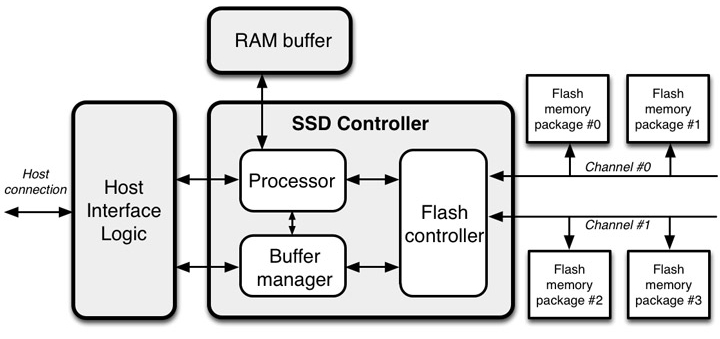
\includegraphics[width=0.8\textwidth]{figure/background/ssd_arch}
	\caption{A simplified diagram of typical SSD.}
	\label{fig:ssd_arch}
\end{figure*}

Figure~\ref{fig:ssd_arch} shows a simplified diagram of typical NAND flash-based storage
devices, consisting of a processor, flash controller, several flash memory packages, and
host interface logic. The FTL running on the processor receives host commands (e.g., reads
and writes) through the host interface module from the host system, and then issues several
flash I/O commands to the flash controller. The flash controller handles multiple I/O commands
simultaneously. Thus, it is possible to achieve much higher performance than utilizing
a single NAND flash chip, providing the aggregate bandwidth of multiple flash chips
with the host system.

\section{Multi-stream Interface}
At the heart of the garbage collection problems of SSD are the issues of
how to predict the lifetime of data written to the SSD and
how to ensure that data with similar lifetime are placed in
the same erase unit. Kang et. al.~\cite{MultiStream}, proposed multi-streaming,
an interface that directly guides data placement within
the SSD, separating the two issues. Authors argue that the
host system should (and can) provide adequate information
about data lifetime to the SSD. It is the responsibility
of the SSD, then, to place data with similar lifetime (as
dictated by the host system) into the same erase unit.

The design introduces the concept of stream. A stream
is an abstraction of SSD capacity allocation that stores a
set of data with the same lifetime expectancy. An SSD
that implements the proposed multi-stream interface allows
the host system to open or close streams and write to
one of them. Before writing data, the host system opens
streams (through special SSD commands) as needed.
Both the host system and the SSD share a unique stream
ID for each open stream, and the host system augments
each write with a proper stream ID. A multi-streamed
SSD allocates physical capacity carefully, to place data
in a stream together and not to mix data from different
streams.


Figure~\ref{fig:multistream} shows the example of block allocation with and without
multi-stream. Without Multi-stream, data are written in the order in which 
they are received. As a result, different lifetimes of data are mixed in the same block.
It incurs high valid page copy overhead for garbage collection due to the different 
invalidation time.
However, with Multi-stream, data with same lifetime are separated in a different block
so that they are likely to be invalidated together that results low garbage collection overhead.
In order to maximize the effect of the multi-streamed SSD, identifying similar lifetime data
is the most important and difficult.

\begin{figure*}[t]
	\centering
	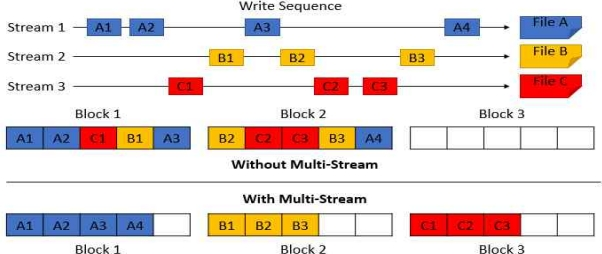
\includegraphics[width=0.8\textwidth]{figure/background/multistream}
	\caption{Block allocation with and without multi-stream.}
	\label{fig:multistream}
\end{figure*}


\section{Inline Data Deduplication Technique}
Inline deduplication saves the lifetime of SSDs more than
offline deduplication~\cite{InlineDedup}. The lifetime of SSD flash cells is limited to a
specified small number of writes and block erasures (e.g., around
5,000 times in MLC SSD). Inline deduplication minimizes the number
of writes to the SSDs by writing only unique data blocks. However,
offline deduplication requires writing all duplicate and unique blocks
to the SSDs first. Then during the idle time, stored data are read, and
the unique ones are written back to respective SSDs.

Inline data deduplication typically consists of four steps. First, the
deduplication module receives a write request with data ($Data_a$)
and logical block address ($LBA_a$). Second, $Data_a$ are chunked into
fixed-sized blocks or variable-sized blocks. In this dissertation, we use
fixed-sized chunking which has a lower CPU utilization requirement
and has been commercially used in primary storage~\cite{InlineDedup}.
Third, the module calculates a signature ($Sig_a$) for the data. Fourth,
the module looks up $Sig_a$ in the deduplication tables. If the
signature matches another signature ($Sig_b$) that was already stored
in the deduplication tables, the received write request is considered
duplicate ($Data_a = Data_b$). Then Dataa will not be written to the
storage devices and the module only updates the deduplication
tables. The update includes recording a mapping from $LBA_a$ to the
physical block address ($PBA_b$) of the matched signature. For cases
that step four cannot find $Sig_a$ in the table, the write request is considered
unique. Therefore, in addition to updating the deduplication
tables, $Data_a$ are written to the storage devices.
%A Scalable HW-Based Inline Deduplication for SSD Arrays

\section{Related Work} 
\subsection{Data Separation Techniques for Multi-streamed SSDs}
There are several research for detecting data temperature. Park, et al.~\cite{multibloom} 
uses multiple bloom
filters to identify hot data in the device layer. Stoica, et al.~\cite{updatefreq}
propose new data placement algorithms to improves
flash write performance by estimating data update frequencies.
Luo, et al.~\cite{writehot} observe high temporal write
locality in different workloads and design a write-hotness
aware retention management policy to improve flash memory
life time. Most research is on a simulation or mathematical
modeling basis and those lack of real world system and
performance analysis. It is hard to guarantee the benefit
of these algorithms in a dynamic I/O intensive datacenter
workloads. In adition, as multi-stream SSDs
become available, there is a need to identify data temperature
and separate them to multiple levels (usually more
than three levels - hot, cold and warm) to fully utilize such
devices.

There have been many studies for multi-streamed SSDs ~\cite{MultiStream, Level,
vStream, FStream, AutoStream, PCStream}.  Kang {\it et al.} first proposed a
multi-streamed SSD that supported manual stream allocation for separating
different types of data~\cite{MultiStream}.  Yang {\it et al.} showed that a
multi-streamed SSD was effective for separating data of append-only
applications like RocksDB~\cite{Level}.  Yong {\it et al.} presented a virtual
stream management technique that allows logical streams, not physical streams,
to be allocated by applications.  Unlike these studies that involve modifying
the source code of target programs, \textsf{\small PCStream} automates the
stream allocation with no manual code modification.

Rho {\it et al.} proposed a stream management technique, called FStream, at the
file system layer~\cite{FStream}. In FStream, metadata, journal
data, and user data that may have different lifetime characteristics were
allocated to separate streams.  Since FStream was implemented as a part of a file
system, it was not able to directly detect application's I/O behaviors.
Also, it may be hard to be deployed in practice due to 
a strong dependence on file system-specific implementation details.
\textsf{\small PCStream}, on the other hand, efficiently exploits
programs' I/O behaviors using PCs with no file system-specific modifications.

Yang {\it et al.} presented an automatic stream management technique at the
block device layer~\cite{AutoStream}. Similar to hot-cold data separation
technique used in FTLs, it approximates the data lifetime of data based on
update frequencies of LBAs.  The applicability of this technique is, however,
quite limited to in-place update workloads only.  \textsf{\small PCStream} has
no such limitation on the workload characteristics, thus effectively working
for general I/O workloads including append-only, write-once 
as well as in-place update workloads.

Ha {\it et al.} proposed an idea of using PCs to separate hot data from cold
one in an FTL layer~\cite{PCHa}.  Kim {\it et al.} extended it for
multi-streamed SSDs~\cite{PCStream}.  Unlike these work, our study treats the
PC-based stream management problem in a more complete fashion by (1)
pinpointing the key weaknesses of existing multi-streamed SSD solutions, (2)
extending the effectiveness of PCs for more general I/O workloads including
write-once patterns, and (3) introducing internal streams as an effective
solution for outlier PCs.  Furthermore, \textsf{\small PCStream} exploits the
globally unique nature of a PC signature for supporting short-lived
applications that runs frequently.



\subsection{Write Traffic Reduction Techniques}
In order to extend the lifetime of flash-based SSDs,
data deduplication techniques have been used in recent SSDs
because they are effective in reducing the amount of data written to flash memory by preventing duplicate data from being written again~\cite{caftl,value-locality}.
As a result, only non-duplicate data, i.e., unique data, are stored in SSDs effectively decreasing the total amount of data written to
SSDs.
In most deduplication schemes proposed for SSDs,
the unit of data deduplication is same as the flash page size which is usually 4 KB or 8 KB.
Using a page as a deduplication unit seems to be reasonable 
because the unit of a read or write operation of flash memory is also a page. 
However, this page-based deduplication technique misses many chances of eliminating duplicate data, especially
when two pages are \textit{almost} identical.
For example, in our experimental analysis of an existing 4 KB page-based deduplication technique, we observed that
up to 34\% mostly identical data.
If the unit of deduplication were smaller than 4 KB, about 23\% more data could be identified as duplicate data.
%We observed that up to 48\% of unique pages actually contain mostly identical data.
%The existing techniques, however, can not completely eliminate the duplicate segment in those pages 
%since they are considered as unique pages.
Furthermore, it is expected that the effectiveness of the page-based deduplication technique would 
get even worse in future NAND flash memory as the page size of 
flash memory is expected to increase
to a bigger size such as 16 KB~\cite{16kpage}.

%In our observation, many pages are rewritten to flash memory after being modified slightly.
%Thus, the contents of the previous page and the new one are nearly identical.
%{\color{red}In our observation, however,
%this page-based deduplication loses many chances of eliminating duplicate data because of following two reasons.
%( ).}

%In order to extend the limited lifespan, data deduplication technique, which removes redundant data from the workload,
%has been widely adopted in SSDs. 
%In the existing scheme, the size of a chunk, which is used as a unit of redundancy checking and writing, is commonly 
%fixed to the page size of the flash memory to minimize the additional management overhead.
%Using page-sized chunking method, however, slightly modified data chunk can not be determined as duplicated data although
%most of data in the chunk are the same, i.e. \textit{partially matched data}.
%Furthermore, the portion of \textit{partially matched data} is expected to be even significantly larger when the flash page size 
%becomes bigger as the semiconductor technology scales down.
%For example, the page size of initial SLC flash memory was 2KB.%~\cite{2kpage}. 
%The 4KB-sized page has become more common in both industry and research in the late 2000s.%~\cite{4kpage1,4kpage2,4kpage3}. 
%In the early 2010s, the scaling trend has been accelerated so 
%that the flash page size has become 8KB%~\cite{8kpage1,8kpage2} 
%and even 16KB. %~\cite{16kpage}. 
%Under the \textit{large-page} flash memory, the existing deduplication techniques
%for SSDs have unavoidable limitations since the probability of finding pages with an exact match will be significantly low.
%---------------------------------------------

%The most well-known approach that improves the storage lifetime is to optimize flash firmware algorithms. 
%As mentioned previously, 
Because of the ``erase-before-write'' nature of NAND flash memory, 
flash storage devices employ a flash translation layer (FTL) 
that supports address mapping, garbage collection, and wear-leveling algorithms~\cite{FAST}. %~\cite{BAST,FAST,LAST}.
These firmware algorithms incur a lot of extra write/erase operations,
seriously shortening the overall lifetime of a storage device.
For this reason, a large number of studies have been focused on reducing such extra operations to improve the storage 
lifetime.
%The firmware-level optimization has been effective in improving the lifetime of flash-based SSDs. 
However, considering the decreasing lifetime of recent high-density NAND flash memory such as TLC NAND flash memory~\cite{tlc}, %~\cite{mlc1,mlc2}, 
more aggressive lifetime management solutions are required. 

Data deduplication techniques, which are originally developed for backup systems,
are regarded as one of the promising approaches for extending the storage lifetime
because of their ability that reduces the amount of write traffic sent to a storage device.
In deduplication techniques, a chunk is used as an unit of identification and elimination of duplicate data.
%An unit of verification of duplicate and elimination is called chunk in deduplication techniques.
Depending on their chunking strategies, deduplication techniques can be categorized into two types,
fixed-size deduplication and variable-size deduplication.
Fixed-size deduplication divides an input data stream into fixed-size chunks (e.g., pages)~\cite{caftl,value-locality}. %~\cite{caftl,value-locality,idedup}.
Then, it decides if each chunk data is duplicate and prevents duplicate chunks %whose data are already stored in flash memory 
from being rewritten to flash memory.
Unlike fixed-size deduplication, 
the chunk size of variable-size deduplication is not fixed.
Instead, it decides a cut point between chunks using 
a content-defined chunking (CDC) algorithm
which divides the data stream according to the contents~\cite{dedupv1, dong}.

% SSD의 경우 fixed-size dedup을 할 수 밖에 없음을 강조
In general, variable-size deduplication techniques can identify more data as duplicate data than the fixed-size deduplication technique.
Since variable-size deduplication adaptively changes the size of chunks by analyzing the contents of input stream,
duplicate data are more effectively found regardless of their locations.
In spite of its advantages, variable-size deduplication is not commonly used in SSDs because of the following practical limitations.

First, the CDC algorithm often requires relatively high computational power and a large amount of memory space. 
Thus, variable-size deduplication is not appropriate to be employed at the level of 
storage devices where computing and memory resources are constrained. 
Second, the size of remaining unique data after deduplication may vary in variable-size deduplication. 
When writing those data, a complicated scheme for data size management is required 
to form sub-page data chunks to fit in a flash page size, preventing an internal fragmentation. 
For those reasons, most existing deduplication techniques for SSDs employ fixed-size deduplication, 
which is relatively simple and does not require a significant amount of hardware resources.

There are several existing studies for fixed-size deduplication for SSDs. F. Chen~\cite{caftl} proposed CAFTL 
to enhance the endurance of SSDs with a set of acceleration techniques to reduce runtime overhead. 
A. Gupta~\cite{value-locality} also proposed CA-SSD to improve the reliability of SSDs by exploiting the value locality, 
which implies that certain data items are likely to be accessed preferentially. 
In these studies, authors focused on the feasibility of deduplication at SSD level and 
proved its effectiveness rather than improving deduplication itself.

Recently, several deduplication techniques for flash-based storage are proposed. Z. Chen~\cite{order-merge}
proposed OrderMergeDedup which orders and merges the deduplication metadata with data writes to 
realize failure-consistent storage with deduplication.  
W. Li~\cite{cachededup} proposed CacheDedup which integrates deduplication with caching architecture to 
address limited endurance of flash caching by managing data writes and deduplication metadata together, 
and proposing duplication-aware cache replacement algorithms. 
These studies focus on systematic approach such as block layer or flash caching. 
However, this study improves the effect of deduplication in the device-specific domain, 
so the approach of this study is quite different.

Similar to the existing deduplication techniques,
the proposed FineDedup technique is also based on fixed-size deduplication.
Using a smaller deduplication unit,
however, FineDedup improves the likelihood of eliminating duplicate data.
This approach can complement the limitation of existing fixed-size deduplication techniques,
which exhibit a relatively low amount of removed writes 
in comparison with variable-size deduplication.

\subsection{Program Context based Optimization Techniques for Operating Systems}
History-based prediction techniques exploit the principle
that most programs exhibit certain degrees of repetitive
behavior. For example, subroutines in an application are
ckalled multiple times, and loops are written to process a
large amount of data. The challenge in making an accurate
prediction is to link the past behavior (event) to
its future reoccurrence. In particular, predictors need the
program context of past events so that future events about
to occur in the same context can be identified. The more
accurate context information the predictor has about the
past and future events, the more accurate prediction it can
make about future program behavior.

A key observation made in computer architecture is that
a particular instruction usually performs a very unique
task and seldom changes behavior, and thus program instructions
provide a highly effective means of recording
the context of program behavior. Since the instructions
are uniquely described by their program counters (PCs)
which specify the location of the instructions in memory,
PCs offer a convenient way of recording the program context.

One of the earliest predictors to take advantage of the
information provided by PCs is branch prediction. 
The PC of the branch instruction uniquely identifies
the branch in the program and is associated with a particular
behavior, for example, to take or not to take the
branch. Branch prediction techniques correlate the past
behavior of a branch instruction and predict its future behavior
upon encountering the same instruction.

The success in using the program counter in branch
prediction was noticed and the PC information has been
widely used in other predictor designs in computer architecture.
Numerous PC-based predictors have been
proposed to optimize energy~\cite{cacheenergy}, cache management~\cite{cachemngmt}
, and memory prefetching~\cite{memoryprefetching}. 
For example, PCs have been used to accurately predict
the instruction behavior in the processor's pipeline
which allows the hardware to apply power reduction techniques
at the right time to minimize the impact on performance~\cite{cacheenergy}
. In Last Touch Predictor~\cite{cachemngmt}, PCs are
used to predict which data will not be used by the processor
again and free up the cache for storing or prefetching
more relevant data. In PC-based prefetch predictors~\cite{memoryprefetching}
, a set of memory addresses or
patterns are linked to a particular PC and the next set of
data is prefetched when that PC is encountered again.

Moreover, PCC~\cite{PC} considers the opportunity and 
viability of PC-based prediction techniques
in operating systems design. In particular, they consider
the buffer cache management problem, which shares common
characteristics with hardware cache management as
they essentially deal with different levels of the memory
hierarchy.
The basic idea is to separate access streams by the program
context (identified by the function call stack) when the I/O
access is made, with the assumption that a single program
context is likely to access disk files with the same pattern in
the future.

However, none of the existing PC-based approach focus of the storage devices.
They use iterative access characteristics according to the PC 
at the operating system level, e.g., cache management.
Based on our analysis on PCs, program context can be a good candidate 
for optimizing performance and lifetime of SSDs.

\chapter{Fully Automatic Stream Management For Multi-Streamed SSDs Using Program Contexts} 
\label{chap:PCstream}

\section{Overview}

In flash-based SSDs, garbage collection (GC) is inevitable because NAND flash
memory does not support in-place updates.  Since the efficiency of garbage
collection significantly affects  both the performance and lifetime of SSDs,
garbage collection has been extensively investigated so that the garbage
collection overhead can be reduced ~\cite{DAC, WriteAmplification, GCGreedy,
GCVictim, GCTTFlash, HotCold}.  For example, hot-cold separation techniques are
commonly used inside an SSD so that quickly invalidated pages are not mixed
with long-lived data in the same block.   For more efficient garbage
collection, many techniques also exploit host-level I/O access characteristics
which can be used as useful hints on the efficient data separation inside the
SSD~\cite{JiTGC, ShadowGC}.

Multi-streamed SSDs provide a special interface mechanism for a host system,
called streams\footnote{In this paper, we use ``streams'' and ``external
streams'' interchangeably.}, which data separation decisions {\it on the
host level} can be delivered to SSDs~\cite{T10, MultiStream}.  When the host
system assigns two data $D_1$ and $D_2$ to different streams $S_1$ and $S_2$,
respectively, a multi-streamed SSD places $D_1$ and $D_2$ in different blocks,
which belong to $S_1$ and $S_2$, respectively.  When $D_1$ and $D_2$ have
distinct update patterns, say, $D_1$ with a short lifetime and $D_2$ with a
long lifetime, allocating $D_1$ and $D_2$ to different streams can be helpful
in minimizing the copy cost of garbage collection by separating hot data from
cold data.  Since data separation decisions can be made more intelligently on
the host level over on the SSD level, when streams are properly managed, they
can significantly improve both the performance and lifetime of flash-based
SSDs~\cite{MultiStream, Level,vStream, FStream, AutoStream}.  We assume that a
multi-streamed SSD supports $m$+1 streams, $S_0$, ..., $S_{m}$.

In order to maximize the potential benefit of multi-streamed SSDs in practice,
several requirements need to be satisfied both for stream management and for
SSD stream implementation.  First, stream management should be supported in a
fully automatic fashion over general I/O workloads without any manual work.
For example, if an application developer should manage stream allocations {\it
manually} for a given SSD, multi-streamed SSDs are difficult to be widely
employed in practice.   Second, stream management techniques should have no
dependency on the number of available streams.  If stream allocation decisions
have some dependence on the number of available streams,  stream allocation
should be modified whenever the number of streams in an SSD changes.  Third,
the number of streams supported in an SSD should be sufficient to work well
with multiple concurrent I/O workloads.  For example, with 4 streams, it would
be difficult to support a large number of I/O-intensive concurrent tasks.  

Unfortunately, to the best of our knowledge, no existing solutions  for
multi-streamed SSDs meet all these requirements.  Most existing
techniques~\cite{MultiStream, Level, vStream, FStream} require programmers to
assign streams at the application level with manual code modifications.
\textsf{\small AutoStream}~\cite{AutoStream} is the only known automatic
technique that supports stream management in the kernel level without manual
stream allocation.  However, since \textsf{\small AutoStream} predicts data
lifetimes using the update frequency of the logical block address (LBA), it
does not work well with append-only workloads (such as
RocksDB~\cite{RocksDB} or Cassandra~\cite{Cassandra})
and write-once workloads (such as a Linux kernel build).  Unlike conventional
in-place update workloads where data written to the same LBAs often show strong update
locality, append-only or write-once workloads make it impossible to predict data lifetimes
from LBA characteristics such as the access frequency.

In this paper, we propose a {\it fully-automatic} stream management technique,
called \textsf{\small PCStream}, which works efficiently over general I/O
workloads including append-only, write-once as well as in-place update workloads.   
The key insight behind
\textsf{\small PCStream} is that stream allocation decisions should be made at
a higher abstraction level where {\it I/O activities}, not LBAs, can be
meaningfully distinguished.  For example, in RocksDB, if we can tell whether
the current I/O is a part of a logging activity or a compaction activity, stream
allocation decisions can be made a lot more efficiently over when only LBAs of
the current I/O is available.   

In \textsf{\small PCStream}, we employ a write program context\footnote{
Since we are interested in write-related system calls such as {\tt write()} in
Linux, we use {\it write program contexts} and {\it program contexts}
interchangeable where no confusion arises.} as such a higher-level
classification unit for representing I/O activity regardless of the type of I/O
workloads.  A program context (PC)~\cite{PC, PC2}, which uniquely represents an
execution path of a program up to a write system call, is known to be effective
in representing dominant I/O activities~\cite{PCHa}.  Furthermore, most
dominant I/O activities tend to show distinct data lifetime characteristics.
By identifying dominant I/O activities using program contexts during run time,
\textsf{\small PCStream} can automate the whole process of stream allocation
within the kernel with no manual work.  In order to seamlessly support various
SSDs with different numbers of streams, \textsf{\small PCStream} groups program
contexts with similar data lifetimes depending on the number of supported
streams using the k-means clustering algorithm~\cite{kmeans}.  Since program
contexts focus on the semantic aspect of I/O execution as a lifetime
classifier, not on the low-level details such as LBAs and access patterns,
\textsf{\small PCStream} easily supports different I/O workloads regardless of
whether it is update-only or append-only.   

Although many program contexts show that their data lifetimes are narrowly
distributed, we observed that this is not necessarily true because of several
reasons.  For example, when a single program context handles multiple types of
data with different lifetimes, data lifetime distributions of such program
contexts  have rather large variances.  In \textsf{\small PCStream}, when such
a program context {\it $PC_j$} is observed (which was mapped to a stream {\it
$S_k$}), the long-lived data of {\it $PC_j$} are moved to a different stream
{\it $S_{k'}$} during GC.  The stream {\it $S_{k'}$} prevents the long-lived
data of the stream {\it $S_k$} from being mixed with future short-lived data of
the stream {\it $S_k$}.

When several program contexts have a large variance in their data lifetimes,
the required number of total streams can quickly increase to distinguish data
with different lifetimes.
%if streams can efficiently distinguish data with different lifetimes.
In order to effectively increase the number of streams, we propose a new stream
type, called an internal stream, which can be used only for garbage collection.
Unlike external streams, internal streams can be efficiently implemented at low
cost without increasing the SSD resource budget.  In the current version of
\textsf{\small PCStream}, we create the same number of internal streams as the
external streams, effectively doubling the number of available streams. 

In order to evaluate the effectiveness of \textsf{\small PCStream}, we have
implemented \textsf{\small PCStream} in the Linux kernel (ver. 4.5) and
extended a Samsung PM963 SSD to support internal streams.  Our experimental
results show that \textsf{\small PCStream} can reduce the GC overhead as much
as a manual stream management technique while requiring no code modification.
Over \textsf{\small AutoStream}, \textsf{\small PCStream} improves the average
IOPS by 28\% while reducing the average WAF by 49\%.


\section{Motivation}
\subsection{No Automatic Stream Management for General I/O Workloads}
%\subsection{\note{No Automatic Stream Management}}
Most existing stream management techniques~\cite{MultiStream,Level,vStream} 
require programmers to manually allocate streams for their applications.
For example, 
in both \textsf{\small ManualStream\footnote{For brevity, we denote the manual stream allocation
method used in ~\cite{MultiStream} by \textsf{\scriptsize ManualStream}.}}~\cite{MultiStream} and 
~\cite{Level}, there is no systematic guildeline on how to
allocate streams for a given application. 
The efficiency of stream allocations largely depends on the programmer's 
understanding and expertise on data temperature ({\it i.e.}, frequency of updates)
and internals of database systems.
Furthermore, many
techniques also assume that the number of streams is known {\it a priori}.  
Therefore, when an SSD with a different number of streams is used, 
these techniques need to re-allocate streams manually.
\textsf{\small vStream}~\cite{vStream} 
is an exception to this 
restriction by allocating streams to virtual streams, not external streams.  
However, even in \textsf{\small vStream}, virtual stream allocations are left to
programmer's decisions.

Although \textsf{\small FStream}~\cite{FStream} and \textsf{\small AutoStream}~\cite{AutoStream}
may be considered 
as automatic stream management techniques,
their applicability is quite limited.
\textsf{\small FStream}~\cite{FStream} can be useful for separating file system metadata but it does not
work for the user data separation.
\textsf{\small AutoStream}~\cite{AutoStream} is the only known technique that works in a 
fully automatic fashion by making stream allocation decisions within 
the kernel.
However, since \textsf{\small AutoStream} predicts data lifetimes using the
access frequency of the same LBA, \textsf{\small AutoStream} does not work well 
when no apparent {\it locality} on LBA accesses exists in applications.  
For example, in recent data-intensive applications 
such as RocksDB~\cite{RocksDB} and Cassandra~\cite{Cassandra}, 
majority of data are written in an append-only manner,
thus no LBA-level locality can be detected inside an SSD.

\begin{figure*}[t]
	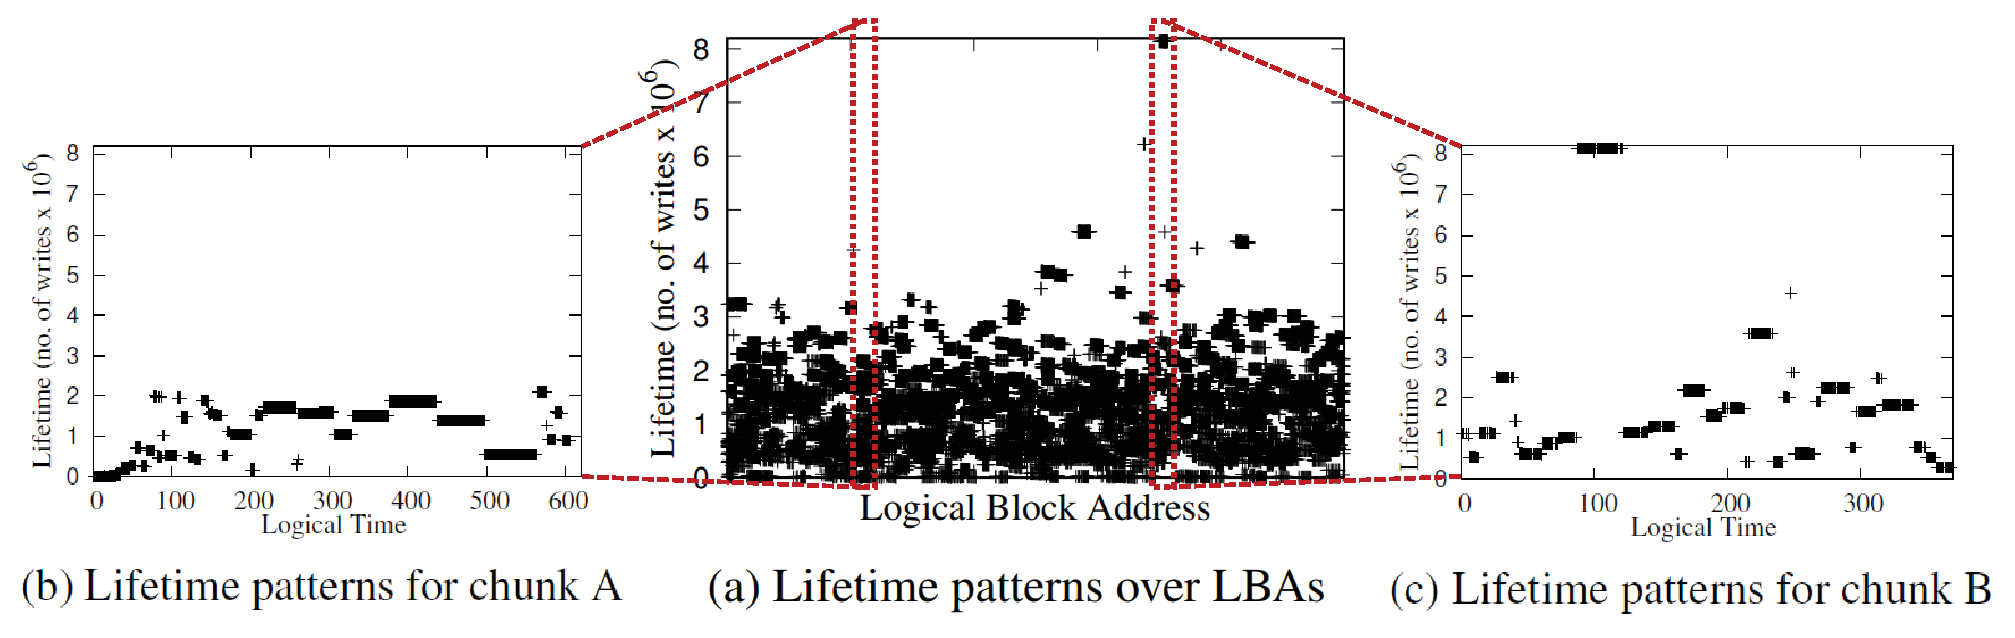
\includegraphics[width=\linewidth]{figure/pcstream/fig1}
	\caption{Lifetime distributions of append-only workload over addresses and times.}
	\label{fig:lba_lifetime}
\end{figure*}


In order to illustrate a mismatch between an LBA-based data separation technique and 
append-only workloads, we analyzed the write pattern of 
RocksDB~\cite{RocksDB}, which is a
popular key-value store based on the LSM-tree algorithm~\cite{LSM}.
Fig.~\ref{fig:lba_lifetime}(a) shows how LBAs may be related 
to data lifetimes in RocksDB.  
We define the lifetime of data as the interval length (in terms of
the logical time based on the number of writes) between
when the data is first written and when the data is invalidated
by an overwrite or a TRIM command~\cite{TRIM}.
As shown in Fig.~\ref{fig:lba_lifetime}(a), 
there is no strong correlation between LBAs and their lifetimes in RocksDB.  

We also analyzed 
if the lifetimes of LBAs change under some predictable patterns over time 
although the overall lifetime distribution shows large variances.
Figs.~\ref{fig:lba_lifetime}(b) and~\ref{fig:lba_lifetime}(c) show
scatter plots of data lifetimes over the logical time 
for two specific 1-MB chunks with 256 pages. 
As shown in Figs.~\ref{fig:lba_lifetime}(b) and~\ref{fig:lba_lifetime}(c), 
for the given chunk, the lifetime of data written to the chunk 
varies in an unpredictable fashion.  
For example, at the logical time 10 in Fig.~\ref{fig:lba_lifetime}(b), 
the lifetime was 1 but it increases about 
2 million around the logical time 450 
followed by a rapid drop around the logical time 500. 
Our workload analysis using RocksDB strongly suggests that under append-only workloads, 
LBAs are not useful in predicting data lifetimes reliably.
In practice, the applicability of LBA-based data separation techniques is quite 
limited to a few cases only when the LBA access
locality is obvious in I/O activities such as updating metadata files or log files.  
In order to support {\it general} I/O workloads in an automatic fashion, stream 
management decisions should be based on higher-level information
which do not depend on lower-level details such as write patterns based on LBAs.

\subsection{Limited Number of Supported Streams}
\label{sec:limitedstreams}

\begin{figure*}[t]
	\centering
	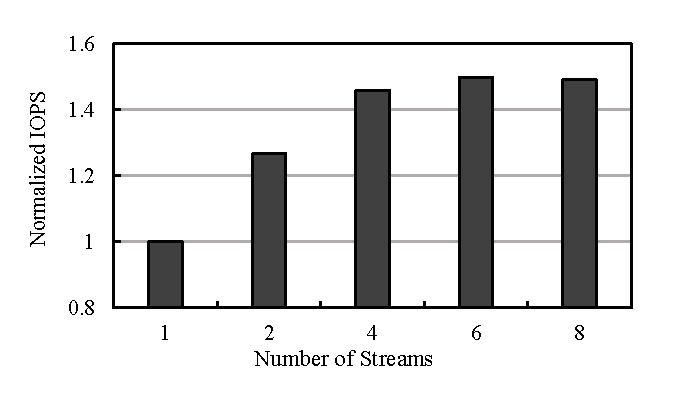
\includegraphics[width=0.8\textwidth]{figure/pcstream/stream_perf}
	\caption{IOPS changes over the number of streams.}
	\label{fig:stream_perf}
\end{figure*}

One of the key performance parameters in multi-streamed SSDs is the number of
available streams in SSDs.  Since the main function of  streams is to separate
data with different lifetimes so that they are not mixed in the same block, it
is clear that the higher the number of streams, the more efficient the
performance of multi-streamed SSDs.  For example, Fig.~\ref{fig:stream_perf}
shows how IOPS in RocksDB changes as the number of streams increases on a
Samsung PM963 multi-streamed SSD with 9 streams.  The \texttt{db\_bench}
benchmark was used for measuring IOPS values with streams manually allocated.
As shown in Fig.~\ref{fig:stream_perf}, the IOPS is continuously improving
until 6 streams are used when dominant I/O activities with different data
lifetimes are sufficiently separated.  In order to support a large number of
streams, both the SBC-4 and NVMe revision 1.3, which define the multi-stream
related specifications, allow up to 65,536 streams~\cite{T10, NVMe}.  However,
the number of streams supported in commercial SSDs is quite limited, say, 4 to
16~\cite{MultiStream, Level, AutoStream}, because of several implementation
constraints on the backup power capacity and fast memory size.

These constraints are directly related to a write buffering mechanism that is
commonly used in modern SSDs.   In order to improve the write throughput while
effectively hiding the size difference between the FTL mapping unit and the
flash program unit, host writes are first buffered before they are written to
flash pages in a highly parallel fashion for high performance.  Buffering host
writes temporarily inside SSDs, however, presents a serious data integrity risk
for storage systems when a sudden power failure occurs.  In order to avoid such
critical failures, in data centers or storage servers where multi-streamed SSDs
are used, SSDs use tantalum or electrolytic capacitors as a backup power
source.  When a main power is suddenly failed, the backup power is used to
write back the buffered data reliably.  Since the capacity of backup power is
limited because of the limited PCB size and its cost, the maximum amount of
buffered data is also limited.  In multi-streamed SSDs where each stream needs
its own buffered area, the amount of buffered data increases as the number of
streams increases.  The practical limit in the capacity of backup power,
therefore, dictates the maximum number of streams as well.

The limited size of fast memory, such as TCM~\cite{TCM} or SRAM, is another
main hurdle in increasing the number of streams in multi-streamed SSDs.  Since
multi-stream related metadata which includes data structures for write
buffering should be accessed quickly as well as frequently, most SSD
controllers implement data structures for supporting streams on fast memory
over more common DRAM.  Since the buffered data is the most recent one for a
given LBA, each read request needs to check if the read request should be
served from the buffered data or not.  In order to support a quick checkup of
buffered data, probabilistic data structures such as a bloom filter can be used
along with other efficient data structures, for accessing LBA addresses of
buffered data and for locating buffer starting addresses.   Since the latency
of a read request depends on how fast these data structures can be accessed,
most SSDs place the buffering-related data structure on fast memory.
Similarly, in order to quickly store buffered data in flash chips, these data
structure should be placed on fast memory as well.  However, most SSD
manufacturers are quite sensitive in increasing the size of fast memory because
it may increase the overall SSD cost.   A limited size of fast memory,
unfortunately, restricts the number of supported streams quite severely.

\section{Automatic I/O Activity Management}
\label{sec:programcontext}
In developing an efficient data lifetime separator for general I/O workloads,
our key insight was that in most applications, the overall I/O behavior of
applications is decided by a few dominant I/O activities ({\it e.g.}, logging and
flushing in RocksDB).  Moreover, data written by dominant I/O activities tend
to have distinct lifetime patterns.  Therefore, if such dominant I/O activities
of applications can be automatically detected and distinguished each other in
an LBA-{\it oblivious} fashion, an automatic stream management technique can be
developed for widely varying I/O workloads including append-only workloads.

In this paper, we argue that a program context can be used to build an
efficient general-purpose classifier of dominant I/O activities with different
data lifetimes.  Here, a PC represents an execution path of an application
which invokes write-related system call functions such as {\tt write()} and
{\tt writev()}.  There could be various ways of extracting PCs, but the most
common approach~\cite{PC, PC2} is to represent each PC with its PC signature
which is computed by summing program counter values of all the functions along
the execution path which leads to a write system call.

%we represent the PC by summing program counter values of
%all the functions along the execution path which leads to a write system call.

%\subsection{Program Context as a Unit of Lifetime Classification}
\subsection{PC as a Unit of Lifetime Classification for General I/O Workloads}
In order to illustrate that using PCs is an effective way to distinguish I/O
activities of an application and their data lifetime patterns, we measured data
lifetime distributions of PCs from various applications with different I/O
workloads.  In this section, we report our evaluation results for three
applications with distinct I/O activities: RocksDB~\cite{RocksDB},
SQLite~\cite{SQLite}, and GCC~\cite{GCC}.  RocksDB shows the append-only
workload while SQLite shows a workload that updates in place.  Both database
workloads are expected to have distinct I/O activities for writing log files
and data files.  GCC represents an extensive compiler workload ({\it e.g.},
compiling a Linux kernel) that generates many short-lived temporary files ({\it
e.g.}, \texttt{.s}, \texttt{.d}, and \texttt{.rc} files) as well as some
long-lived files ({\it e.g.}, object files and kernel image files).

%\textcolor{red}{(TODO: 갑자기
%lifetime 이야기가 나옴. 없애도 큰 문제가 없을 듯...) \sout{Note that using a
%program context to distinguish data lifetimes is not new. For example, Ha {\it
%et al.} proposed a data separation technique based on the program
%context~\cite{PCHa}.  However, their work was neither designed for append-only
%workloads nor for modern multi-streamed SSDs.}}

\begin{figure*}[!t]
\centering
	\subfloat[RocksDB: Logging]{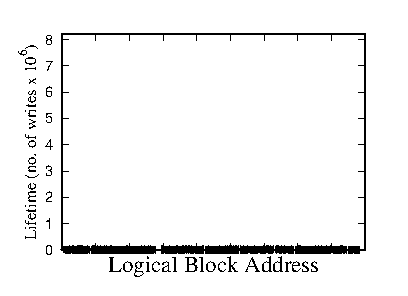
\includegraphics[width=0.3\textwidth]{figure/pcstream/pcID_2_new.eps}} % data from 4/03031953 
	\hspace{2pt}
	\subfloat[RocksDB: Flushing]{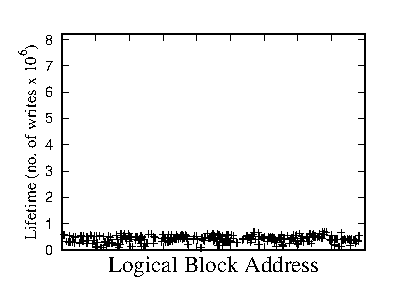
\includegraphics[width=0.3\textwidth]{figure/pcstream/pcID_3_new.eps}}
	\hspace{2pt}
	\subfloat[RocksDB: Compaction]{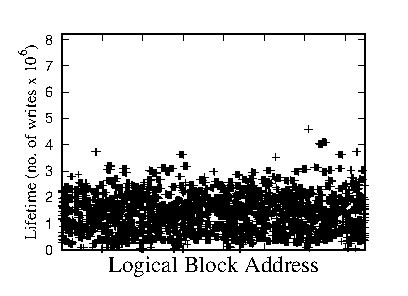
\includegraphics[width=0.3\textwidth]{figure/pcstream/pc_3_new.eps}}  % data from 4/03040047
	\hfill
	\subfloat[SQLite: Logging]{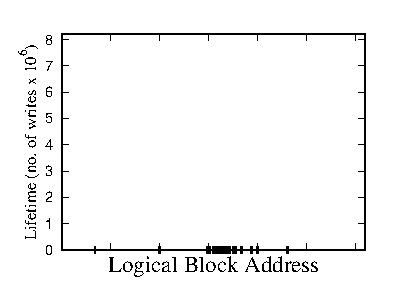
\includegraphics[width=0.3\textwidth]{figure/pcstream/sqlite_pcID_6_new.eps}}
	\hspace{2pt}
	\subfloat[SQLite: Updating]{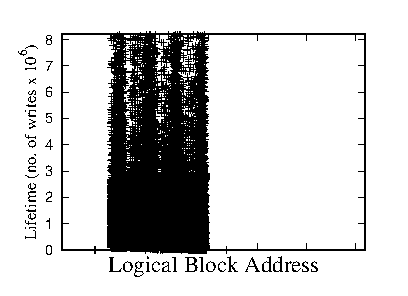
\includegraphics[width=0.3\textwidth]{figure/pcstream/sqlite_pcID_1_new.eps}}
	\hspace{2pt}
	\subfloat[GCC: Outputting Temp]{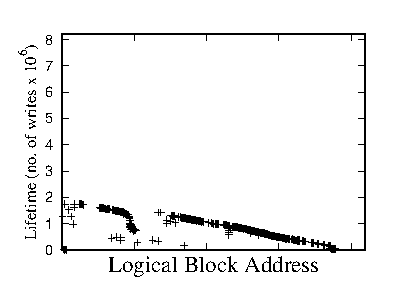
\includegraphics[width=0.3\textwidth]{figure/pcstream/gcc_pcID_1_new.eps}}
	\hfill
	\subfloat[GCC: Outputting Executable]{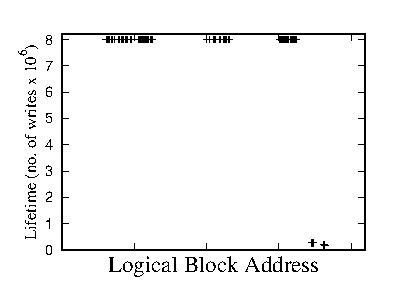
\includegraphics[width=0.3\textwidth]{figure/pcstream/gcc_pcID_8_new.eps}}
\caption{Data lifetime distributions of dominant I/O activities in RocksDB, SQLite and GCC.} 
\label{fig:types_and_PCs}
\end{figure*}


To confirm our hypothesis that data lifetimes can be distinguished by tracking
dominant I/O activities and a PC is a useful unit of classification for
different I/O activities, we have analyzed how well PCs work for RocksDB,
SQLite and GCC.  Fig.~\ref{fig:types_and_PCs} shows data lifetime distributions
of dominant I/O activities which were distinguished by computed PC values.  As
expected, Fig.~\ref{fig:types_and_PCs} validates that dominant I/O activities
show distinct data lifetime distributions over the logical address space.  For
example, as shown in
Figs.~\ref{fig:types_and_PCs}(a)$\sim$\ref{fig:types_and_PCs}(c), the logging
activity, the flushing activity and the compaction activity in RocksDB clearly
exhibit quite different data lifetime distributions.  While the logged data
written by the logging activity have short lifetimes, the flushed data by the
flushing activity have little bit longer lifetimes.  Similarly, for SQLite and
GCC, dominant I/O activities show quite distinct data lifetime characteristics
as shown in Figs.~\ref{fig:types_and_PCs}(d)$\sim$\ref{fig:types_and_PCs}(g).
As shown in Fig.~\ref{fig:types_and_PCs}(d), the logging activity of SQLite
generates short-lived data.  This is because SQLite overwrites logging data in
a small and fixed storage space and then removes them soon.  Lifetimes of
temporary files generated by GCC are also relatively short as shown in
Fig.~\ref{fig:types_and_PCs}(f), because of the write-once pattern of temporary
files.  But, unlike the other graphs in Fig.~\ref{fig:types_and_PCs}, data
lifetime distributions of Figs.~\ref{fig:types_and_PCs}(c) and
\ref{fig:types_and_PCs}(e), which correspond to the compaction activity of
RocksDB and the updating activity of SQLite, respectively, show large
variances.  These {\it outlier I/O activities} need a special treatment, which
will be described in Section~\ref{sec:internal}.

Note that if we used an LBA-based data separator instead of the proposed
PC-based scheme, most of data lifetime characteristics shown in
Fig.~\ref{fig:types_and_PCs} could not have been known.  Only the data lifetime
distribution of the logging activity of SQLite, as shown in
Fig.~\ref{fig:types_and_PCs}(d), can be accurately captured by the LBA-based
data separator.  For example, the LBA-based data separtor cannot decide that
the data lifetime of data produced from the outputting temp activity of GCC is
short because temporary files are not overwritten each time they
are generated during the compiling step. 

\section{Support for Large Number of Streams}
\label{sec:internal}
The number of streams is restricted to a small number 
because of the practical limits on the backup power capacity and the size of fast memory.
Since the number of supported streams critically impacts the overall performance 
of multi-streamed SSDs, in this section, we propose a new type of streams, 
called {\it internal streams}, which can be
supported without affecting the capacity of a backup power as well as 
the size of fast memory in SSDs.   
Internal streams, which are restricted to be used only for garbage collection, 
significantly improve the efficiency of PC-based stream allocation,
especially when PCs show large lifetime variances in their data lifetime
distributions.

%\subsection{Program Contexts with Large Lifetime Variances}
\subsection{PCs with Large Lifetime Variances}
\label{sec:largevariance}
For most PCs, their lifetime distributions tend to have small variances
({\it e.g.}, Figs.~\ref{fig:types_and_PCs}(a), ~\ref{fig:types_and_PCs}(d), and
~\ref{fig:types_and_PCs}(f)).
However, we observed that 
it is inevitable to have a few PCs with large lifetime variances 
because of several practical reasons.
For example, when multiple I/O contexts are covered by the same execution path, 
the corresponding PC may represent several I/O contexts whose data lifetimes are quite different.   
Such a case occurs, for example, 
in the compaction job of RocksDB.
RocksDB maintains
several levels, L1, ..., L$n$, in the persistent storage, except for L0 (or a
memtable) stored in DRAM.  Once one level, say L2, becomes full, all the data
in L2 is compacted to a lower level ({\it i.e.}, L3).  It involves moving data from L2
to L3, along with the deletion of the old data in L2.  In the
LSM tree~\cite{LSM}, a higher level is smaller than a lower level 
({\it i.e.}, the size of (L2) $<$ the size of (L3)). 
Thus, data stored in a higher level is invalidated more frequently than those kept
in lower levels, thereby having shorter lifetimes.

\begin{figure}[!t]
\centering
\subfloat[RocksDB: L2 Compaction]{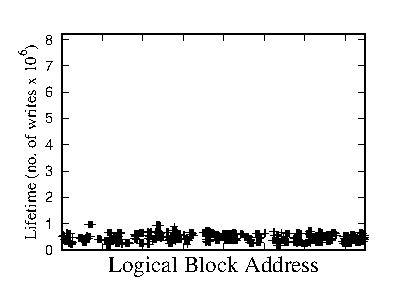
\includegraphics[width=0.4\textwidth]{figure/pcstream/type_4_new.eps}}  % data from 4/03040047
	\hspace{10pt}
\subfloat[RocksDB: L4 Compaction]{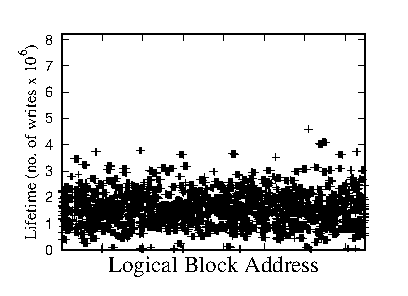
\includegraphics[width=0.4\textwidth]{figure/pcstream/type_6_new.eps}}
%\caption{The lifetime distribution of the compaction activity.} 
\caption{Lifetime distributions of the compaction activity at different levels.} %shane part
\label{fig:compaction}
\end{figure}




Unfortunately, in the current RocksDB implementation, the compaction step is supported 
by the same execution path ({\it i.e.}, the same PC) regardless of the level.
Therefore, the PC for the compaction activity cannot effectively separate data with 
short lifetimes from one with long lifetimes.
Fig.~\ref{fig:compaction}(a) and ~\ref{fig:compaction}(b) show
distinctly different lifetime distributions based on the level of compaction:
data written from the level 4 have a large lifetime variance while data written from
the level 2 have a small lifetime variance.

Similarly, in SQLite and GCC, program contexts with large lifetime variations
are also observed.
Fig.~\ref{fig:types_and_PCs}(e) shows large lifetime variances of data files in
SQLite.
Since client request patterns will decide how SQLite updates its tables, 
the lifetime of data from the updating activity of SQLite is distributed 
with a large variance.  Similarly, the lifetime of
data from the outputting temporary files of GCC can significantly fluctuate 
as well depending on when the next compile step starts.   
Fig.~\ref{fig:types_and_PCs}(g) shows long lifetimes of 
object files/executable files after 
a Linux build was completed
(with no more re-compiling jobs).
However, the lifetime of the same object files/executable files 
may become short when if we have to restart the same
compile step right after the previous one is finished
({\it e.g.}, because of code changes).

For these {\it outlier} PCs with large lifetime variations, 
it is a challenge to allocate streams in an efficient fashion unless 
there are more application-specific hints ({\it e.g.}, the compaction level in
RocksDB) are available.  
As an ad-hoc (but effective) solution, when a PC shows a large variance 
in its data lifetime, we allocate an additional stream, called an internal stream, 
to the PC so that
the data written from the PC can be better separated between the original 
stream and its internal stream.  
In order to support internal streams, the total number of streams may 
need to be doubled so
that each stream can be associated with its internal stream.

\subsection{Implementation of Internal Streams}
As described in Section~\ref{sec:limitedstreams}, it is difficult to increase the number of 
(normal) streams.  However, 
if we restrict that internal streams are used only for data movements
during GC,
they can be quite efficiently
implemented without the constraints on the backup power capacity and fast memory size.  
The key difference in the implementation overhead between normal streams and 
internal streams comes from a simple observation that data copied during 
GC do not need the same reliability and performance support as for host writes.  
Unlike buffered data from host write requests, valid pages in
the source block during garbage collection have no risk of losing their data 
from the sudden power-off conditions because the original valid pages are always available.    
Therefore, even if the
number of internal streams increases, unlike normal streams, 
no higher-capacity backup capacitor is necessary for managing buffered data for internal streams. 

The fast memory requirement is also not directly increased as the number 
of internal streams increases.   
Since internal streams are used only for GC and most GC can be handled as background tasks,
internal streams has a less stringent performance requirement.  
Therefore, data structures for supporting internal streams can be placed 
on DRAM without much performance issues.  
Furthermore, for a read request, there is no need to check if a read request 
can be served by buffered data as in normal streams because the source block always 
has the most up-to-date data.  
This, in turn, allows data structures for internal streams to be located in slow memory.
Once an SSD reaches the fully saturated condition where host writes and GC 
are concurrently performed, the performance of GC may degrade a little because of
the slow DRAM used for internal streams.   
However, in our evaluation, such cases were rarely observed under a 
reasonable overprovisioning storage capacity.


\section{Design and Implementation of \textsf{PCStream}}

\begin{figure}[t]
	\centering
	%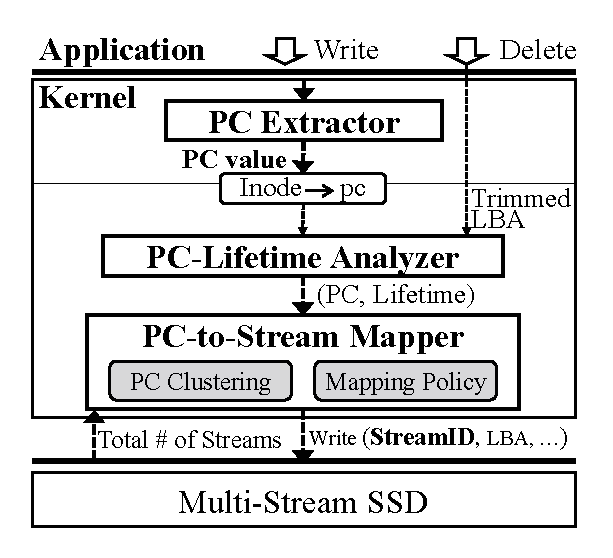
\includegraphics[width=0.6\linewidth]{figure/architecture4}
	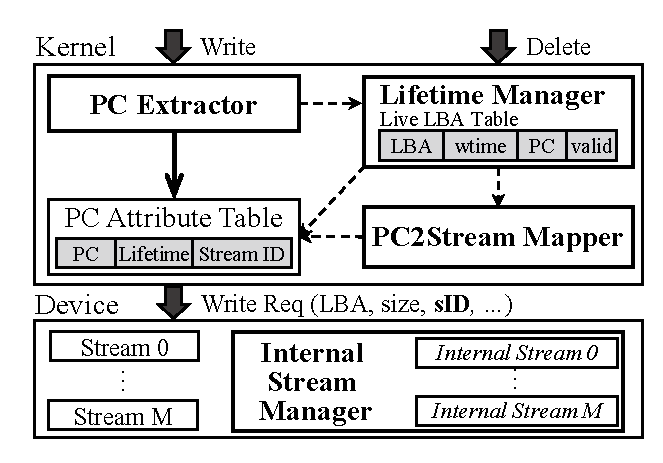
\includegraphics[width=0.8\linewidth]{figure/pcstream/overview_1}
	\caption{An overall architecture of \textsf{\small PCStream}.}
	\label{fig:architecture}
\end{figure}

% stream tbl (X)
% 4.2 -> 5
% short-lived app (X)
% training?

In this section, we explain the detailed implementation of \textsf{\small
PCStream}.  Fig.~\ref{fig:architecture} shows an overall architecture of
\textsf{\small PCStream}. The \textit{PC extractor} is implemented as part of a
kernel's system call handler as already described in
Section~\ref{sec:programcontext}, and is responsible for computing a PC
signature from applications.  The PC signature is used for deciding the
corresponding stream ID\footnote{ We call {\it i} the stream ID of $S_i$.} from
the PC attribute table.  \textsf{\small PCStream} maintains various per-PC
attributes in the PC attribute table including PC signatures, expected data
lifetimes, and stream IDs.  In order to keep the PC attribute table updated
over changing workloads, the computed PC signature with its LBA information is
also sent to the {\it lifetime manager}, which estimates expected lifetimes of
data belonging to given PCs.  Since commercial multi-streamed SSDs only expose
a limited number of streams to a host, the \textit{PC2Stream mapper} groups PCs
with similar lifetimes using a clustering policy, assigning PCs in the same
group to the same stream.  Whenever the lifetime manager or the PC2Stream
mapper are invoked, the PC attribute table is updated with new outputs from
these modules.  Finally, the \textit{internal stream manager}, 
which was implemented inside an SSD as a firmware, is responsible for
handling internal streams associated with external streams.

%the lifetime of data written by write-related system calls can be
%monitored at the program context level.  
%A PC signature value is stored in an
%inode data structure of a file system (modified for \textsf{\small PCStream})
%and is delivered to \textit{the lifetime analyzer module} which estimates
%expected lifetimes of data belonging to a given PC in the block device level.
%In order to efficiently detect the end of data lifetime in append-only
%workloads, the lifetime analyzer also intercepts TRIM~\cite{TRIM} requests from
%a file system.

%shane part Based on the lifetime information, \textit{the PC-to-stream mapper
%module} clusters PCs with similar lifetimes and maps them together to the same
%stream ID.  This mapping is required because the number of streams in an SSD
%is generally less than the number of PCs in host applications.

\subsection{PC Lifetime Management}
\label{sec:PC_lf_mngm}
The responsibility of the lifetime manager is for estimating the lifetime of
data associated with a PC. 
Except for outlier PCs, most data from the same PC tend to show similar 
data lifetimes with small variances.

\textbf{Lifetime estimation:}
Whenever a new write request {\it R} arrives, the lifetime manager stores the
write request time, the PC signature, $PC_i$, and the LBA list of {$R$} into
the live LBA table.  The live LBA table, indexed by an LBA, is used in
computing the lifetime of data stored at a given LBA which belongs to $PC_i$.
Upon receiving TRIM commands (that delete previously written LBAs) or overwrite
requests (that update previously written LBAs), the lifetime manager searches
the live LBA table for a PC signature $PC_{found}$ with the LBA list which
includes the deleted/updated LBAs.  The new lifetime $l_{new}$ of $PC_{found}$
is estimated using the lifetime of the matched LBA from the live LBA table. The
weighted average of the existing lifetime $l_{old}$ for $PC_{found}$ and
$l_{new}$ is used to update the $PC_{found}$ entry in the PC attribute table.
Note that the written time entry of the live LBA table is updated differently
depending on TRIM commands or overwrite requests.  The written time entry
becomes invalid for TRIM while it is updated by the current time for
an overwrite request.

Maintaining the live LBA table, which is indexed by an LBA unit, in DRAM could
be a serious burden owing to its huge size. In order to mitigate the DRAM
memory requirement, the lifetime manager slightly sacrifices the accuracy of
computing LBA lifetime by increasing the granularity of LBA lifetime prediction
to 1 MB, instead of 4 KB.  The live LBA table is indexed by 1 MB LBA, and each
table entry holds PC signatures and written times over a 1 MB LBA range.
Because of the coarse-grained indexing, each entry could have multiple
signatures and written times, and the same PC could span across multiple
entries.  If the same PC has different lifetimes, we take the arithmetic mean
as the PC lifetime.  To limit the table size, if the table reaches a threshold
size, the least recently referenced entry is evicted from the LBA table.
Currently, the threshold is set to 64 MB.

\textbf{PC attribute table:}
The PC attribute table keeps PC signatures and its expected lifetimes. To
quickly retrieve the expected lifetime of a requested PC signature, the PC
attribute table is managed through a hash data structure. Each hash entry
requires only 12 bytes: 64-bit for a PC signature and 32-bit for a predicted
lifetime.  The table size is thus small so that it can be entirely loaded
in DRAM.  From our evaluations, the DRAM size of the PC attribute table was
sufficient with several tens or hundreds of KB.

In addition to the main function of the PC attribute table that maintains the
data lifetime for a PC, the $memory-resident$ PC attribute table has another
interesting benefit for the efficient stream management.  Since a PC
signature of an I/O activity is virtually guaranteed to be {\it globally unique} across
{\it all} applications (the uniqueness property), and a PC signature does not change
over different executions of the same application (the consistency property), the PC
attribute table can capture a long-term history of programs' I/O behaviors.
Because of the uniqueness and consistency of a PC signature, \textsf{\small PCStream}
can exploit the I/O behavior of even short-lived processes ({\it e.g.}, \texttt{cpp}
and \texttt{cc1} for GCC)  that are launched and terminated frequently.  When
short-lived processes are frequently executed, the PC attribute table can hold
their PC attributes from their previous executions, thus enabling quick but
accurate stream allocation for short-lived processes.

The consistency property is rather straightforward because each PC signature is
determined by the sum of return addresses inside a process's virtual address
space.  Unless a program's binary is changed after recompilation, those return
addresses remain the same, regardless of program's execution.  The uniqueness property 
is also somewhat obvious from the observation that the probability that
distinct I/O activities that take different function-call paths have the same
PC signature is extremely low. This is even true for multiple programs. Even
though they are executed in the same virtual address space, it is very unlikely
that I/O activities of diverged programs taking different function-call paths
have the same PC.  Consequently, this immutable property of the PC signature
for a given I/O activity makes it possible for us to characterize the given I/O
activity in a long-term basis without a risk of PC collisions.

%The PC is determined by the sum of the return address, i.e., the path to reach
%the write system call.  In general, different I/O activities can not have the
%same return address because they are implemented in different functions.
%Since the probability that the sum of the different return addresses becomes
%the same is very low, the PC of an I/O activity in the same program is unique.
%For multiple programs, however, since each program uses a virtual address,
%several identical return addresses can occur.  However, the probability that
%two independent programs will have the same function call path over four or
%five is also very low, so we can usually say that a PC is unique.  Moreover,
%since the virtual address of the code is not changed after the compilation,
%the PC value will be the same when the program execution is terminated and
%restarted.  PCs of restarted program will be the same as the one of previous
%execution, and the life characteristics of the PC are also the same.  Because
%PCs are unique, if PC lifetime information is maintained, appropriate stream
%can be allocated even to the first request of a restarting program.

\subsection{Mapping PCs to SSD streams}

After estimating expected lifetimes of PC signatures, the PC2Stream mapper
attempts to group PCs with similar lifetimes into an SSD stream.  This grouping
process is necessary because while commercial SSDs only support a limited
number of streams ({\it e.g.,} 9), the number of unique PCs can be larger ({\it e.g.},
30).  For grouping PCs with similar lifetimes, the PC2Stream mapper module
uses the k-means algorithm~\cite{kmeans} which is widely used for similar
purposes.  In \textsf{\small PCStream}, we use the difference in the data
lifetime between two PCs as a clustering distance and  generates {\it m}
clusters of PCs for $m$ streams.  This algorithm is particularly well suited
for our purpose because it is lightweight in terms of the CPU cycle and
memory requirement.  To quickly assign a proper stream to incoming data, we add
an extra field to the PC attribute table which keeps a stream ID for each PC
signature.  More specifically, when a new write request comes, a designated SSD
stream ID is obtained by referring to the PC attribute table using request's PC
value as an index.  If there is no such a PC in the table, or a PC does not
have a designated stream ID, the request gets default stream ID, which is set
to 0.

For adapting to changing workloads, re-clustering operations should be
performed regularly. This re-clustering process is done in a straightforward
manner. The PC2Stream mapper scans up-to-date lifetimes for all PCs in the PC
attribute table. Note that PC's lifetimes are updated whenever the lifetime
manager gets new lifetimes while handling overwrites or TRIM requests, as
explained in Section~\ref{sec:PC_lf_mngm}.  With the scanned information, the PC2Stream mapper
recomputes stream IDs and updates stream fields of the PC attribute table.  In
order to minimize unnecessary overhead of frequent re-clustering operations,
re-clustering is triggered when 10\% of the PC lifetime entries in the PC
attribute table is changed.


\subsection{Internal Stream Management}
As explained in Section~\ref{sec:largevariance}, there are a few outlier PCs with large lifetime
variances. In order to treat these PCs in an efficient fashion, we devise a
two-phase method that decides SSD streams in two levels: the main stream in the
host level and its internal stream in the SSD level.  Conceptually, long-lived
data in the main stream are moved to its internal stream so that (future)
short-lived data will not be mixed with long-lived data in the main stream.
Although moving data to the internal stream may increase WAF, the overhead can
be hidden if we restrict data copies to the internal stream during GC only.
Since long-lived data ({\it i.e.}, valid pages) in a victim block are moved to a free
block during GC, blocks belong to an internal stream tend to contain long-lived
data.  For instance, \textsf{\small PCStream} assigns the compaction-activity
{\it $PC_1$} to a main stream {\it $S_1$} in the first phase.  To separate the
long-lived data of {\it $PC_1$} ({\it e.g.}, L4 data) from future short-lived data of
the same {\it $PC_1$} ({\it e.g.}, L1 data), valid pages of the {\it $S_1$} are
assigned to its internal stream for the second phase during GC.

We have implemented the internal stream manager with the two-phase method in
Samsung's PM963 SSD~\cite{PM963}. To make it support the two-phase method, we
have modified its internal FTL so that it manages internal streams while
performing GC internally.  Since the internal stream manager assigns blocks for
an internal stream and reclaims them inside the SSD, no host interface changed
is required.

%{\color{blue} 추가로, SSD가 지원하는 stream의 개수가 변경되는 상황에서도
%reclustering을 통해
%대응이 가능하다.
%reclustering의 주기는 workload의 변화 패턴에 따라 결정될 수 있다.
%새로운 PC가 계속적으로 생성되거나 한 PC의 수명 패턴이 자주 변화할 경우 reclustering의 주기를 
%좀 더 짧게 설정하여 workload 변화를 반영한다.
%}
%Since the
%number of PCs created by applications is not limited, the clustering algorithm
%must be efficient enough to quickly handle many PCs. 

\subsection{PC Extraction for Indirect Writes}
One limitation of using PCs to extract I/O characteristics is that it only
works with C/C++ programs that \textit{directly} call write-related system
calls.  Many programs, however, often invoke write system calls
\textit{indirectly} through intermediate layers, which makes it difficult to
track program contexts.

The most representative example may be Java programs, such as Cassandra, that
run inside a Java Virtual Machine (JVM). Java programs invoke write system
calls via the Java Native Interface (JNI)~\cite{JNI} that enables Java programs
to call a native I/O library written in C/C++.  For Java programs, therefore, the
PC extractor shown in Fig.~\ref{fig:architecture} fails to capture Java-level
I/O activities as it is unable to inspect the JVM stack from the native write
system call which is indirectly called through the JNI.  Another example is a
program that maintains a write buffer that is dedicated to dealing with all the
writes from an application. For example, in MySQL~\cite{MySQL} and
PostgreSQL~\cite{PostgreSQL}, every write is first sent to a write buffer.
Separate flush threads later materialize buffered data to persistent storage.
In that case, the PC extractor only captures PCs of flush threads, not PCs of
I/O activities that originally generate I/Os, because the I/O activities were
executed in different threads using different execution stacks.

\begin{figure}[t]
\centering
	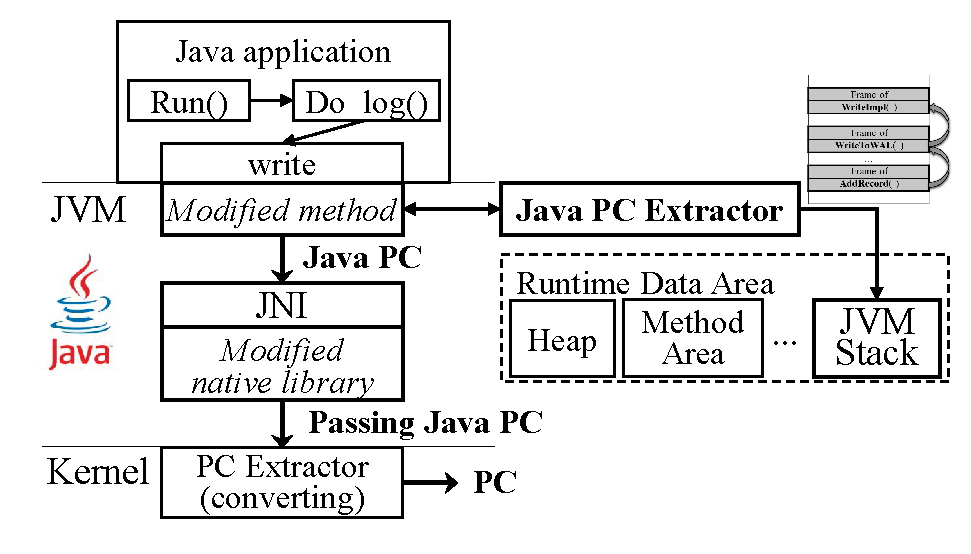
\includegraphics[width=0.7\linewidth]{figure/pcstream/jvmpc}
	\caption{Extracting PCs for JVM.}
\label{fig:java}
\end{figure}

The problem of indirect writes can be addressed by collecting PC signatures
{\it at the front-end interface} of an intermediate layer that accepts write
requests from other parts of the program. In case of Java programs, a native
I/O library can be modified to capture write requests and computes their PC
signatures. Once a native library is modified, \textsf{\small PCStream} can
automatically gather PC signatures without modifying application programs.
Fig.~\ref{fig:java} illustrates how \textsf{PCStream} collects PC signatures
from Java programs.  We have modified the OpenJDK~\cite{OpenJDK} source to
extract PC signatures for most of write methods in write related classes, such
as \texttt{OutputStream}.  The stack area in the \texttt{Runtime Data Areas} of
JVM is used to calculate PC signatures.  The calculated PC is then passed to
the write system call of the kernel via the modified native I/O libraries.

Unlike Java, there is no a straightforward way to collect PCs from applications
with write buffers. This is because the implementation of write buffering is
different depending on applications. Additional efforts to manually modify code
are unavoidable. However, the scope of this manual modification is limited only
to the write buffering code, and application logics themselves don't need to be
edited or annotated.


\section{Experimental Results}
\subsection{Experimental Settings}
In order to evaluate \textsf{\small PCStream}, we have implemented it in the
Linux kernel (version 4.5) on a PC host with Intel Core i7-2600 8-core
processor and 16~GB DRAM.  As a multi-streamed SSD, we used Samsung's PM963
480~GB SSDs.  The PM963 SSD supports up to 9 streams; 8 user-configurable
streams and 1 default stream.  When no stream is specified with a write
request, the default stream is used.  To support internal streams, we have
modified the existing PM963 FTL firmware.  For a detailed performance analysis,
we built a modified {\tt nvme-cli}~\cite{nvmecli} tool that can retrieve the internal
profiling data from \textsf{\small PCStream}-enabled SSDs.  
Using the modified {\tt nvme-cli} tool, we can monitor 
WAF values and per-block data lifetimes from the extended PM963 SSD during run time.

We compared \textsf{\small PCStream} with three existing schemes:
\textsf{\small Baseline}, \textsf{\small ManualStream}~\cite{MultiStream}, and
\textsf{\small AutoStream}~\cite{AutoStream}.  \textsf{\small Baseline}
indicates a legacy SSD that does not support multiple streams. \textsf{\small
ManualStream} represents a multi-streamed SSD with manual stream allocation.
\textsf{\small AutoStream} represents the LBA-baed stream management technique
proposed in ~\cite{AutoStream}. 


We have carried out experiments with various benchmark programs
which represent distinct write characteristics.
RocksDB~\cite{RocksDB} and Cassandra~\cite{Cassandra} have
append-only write patterns. SQLite~\cite{SQLite} has in-place update write patterns
and GCC~\cite{GCC} has write-once patterns.  
For more realistic evaluations, we also used mixed workloads running two 
different benchmark programs simultaneously.

In both RocksDB and Cassandra experiments, Yahoo! Cloud Serving Benchmark
(YCSB)~\cite{YCSB} with 12-million keys was used to generate update-heavy
workloads (workload type A) which consists of 50/50 reads and writes.  Since
both RocksDB and Cassandra are based on the append-only LSM-tree
algorithm~\cite{LSM}, they have three dominant I/O activities (such as logging,
flushing, and compaction).  Cassandra is written in Java, so its PC is
extracted by the modified procedure described in Section~\ref{sec:internal}.  In SQLite evaluations,
TPC-C~\cite{TPCC} was used with 20 warehouses.  SQLite has two dominant I/O
activities such as logging and updating tables.  In GCC experiments, a Linux
kernel was built 30 times.  For each build, 1/3 of source files, which were
selected randomly, were modified and recompiled.  Since GCC creates many
temporary files ({\it e.g.}, \texttt{.s}, \texttt{.d}, and \texttt{.rc}) as
well as long-lived files ({\it e.g.}, \texttt{.o}) from different compiler
tools, there are more than 20 dominant PCs.  To generate mixed workloads, we run
RocksDB and GCC scenarios together (denoted by Mixed 1), and run SQLite and GCC
scenarios at the same time (denoted by Mixed 2).  In order to emulate an aged
SSD in our experiments, 90\% of the total SSD capacity was initially filled up
with user files before benchmarks run.

\subsection{Performance Evaluation}

\begin{figure}[t]
	\centering
	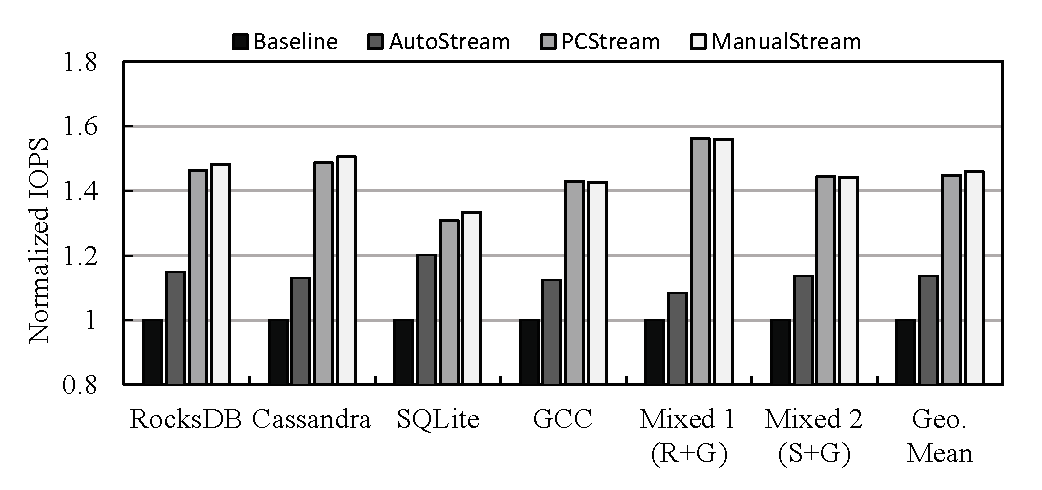
\includegraphics[width=1\linewidth]{figure/pcstream/iops}
	\caption{A comparison of normalized IOPS.}
	\label{fig:iops}
\end{figure}

We compared IOPS values of three existing techniques with \textsf{\small
PCStream}.  Fig.~\ref{fig:iops} shows normalized IOPS for six benchmarks with
four different techniques. For all the measured IOPS values\footnote{ For
RocksDB, Cassandra, and SQLite, the YCSB benchmark and TPC-C benchmark compute
IOPS values as a part of the benchmark report.  For GCC,
where an IOPS value is not measured during run time, 
we computed the IOPS value as a ratio between the total number of write requests
(measured at the block device layer) and the total elapsed time of running GCC.},
\textsf{\small PCStream} improved the average IOPS by 45\% and 28\% over 
\textsf{\small Baseline} and \textsf{\small AutoStream}, respectively.
\textsf{\small PCStream} outperformed \textsf{\small AutoStream}
by up to 56\% for complex workloads ({\it i.e.}, GCC, Mixed1 and Mixed 2) where
the number of extracted PCs far exceeds the number of supported streams
in PM963. The high efficiency of \textsf{\small PCStream} under complex
workloads comes from two novel features of \textsf{\small PCStream}: (1) LBA-oblivious 
PC-centric data separation and (2) a large number of streams supported 
using internal streams. \textsf{\small AutoStream}, on the other hands,
works poorly except for SQLite where the LBA-based separation
can be effective.
Even in SQLite, \textsf{\small PCStream} outperformed \textsf{\small AutoStream}
by 10\%.

\subsection{WAF Comparison}

Fig.~\ref{fig:waf} shows WAF values of four techniques for six benchmarks.
Overall, \textsf{\small PCStream} was as efficient as \textsf{\small
ManualStream}; Across all the benchmarks, \textsf{\small PCStream} showed 
similar WAF values as \textsf{\small ManualStream}. \textsf{\small PCStream}
reduced the average WAF by 63\% and 49\% over \textsf{\small Baseline} and
\textsf{\small AutoStream}, respectively.  

As expected, \textsf{\small Baseline} showed the worst performance among all
the techniques. Owing to the intrinsic limitation of LBA-based data
separation, \textsf{\small AutoStream} performs poorly except for
SQLite.  Since \textsf{\small PCStream} (and \textsf{\small ManualStream}) did
not depend upon LBAs for stream separations, they performed well consistently,
regardless of write access patterns. As a result, \textsf{\small PCStream}
reduced WAF by up to 69\% over \textsf{\small AutoStream}.

%Only SQLite had in-place update patterns for log files, 
%but the larger amount of data were written to database files 
%whose lifetimes are determined by the client
%which makes hard to predict their lifetime by the address.  In PCStream,
%however, long-lived data in database files are moved to internal streams during
%GC so that we can further reduce WAF.

One interesting observations in Fig.~\ref{fig:waf} is that \textsf{\small
PCStream} achieved a lower WAF value than even \textsf{\small ManualStream} for
GCC, Mixed 1, and Mixed 2 where more than the maximum number of streams in
PM963 are needed.  In \textsf{ManualStream}, DB applications and GCC were
manually annotated at offline, so that write system calls were statically bound
to specific streams during compile time.  When multiple programs run together
as in three complex workloads ({\it i.e.}, GCC, Mixed 1 and Mixed 2), static stream
allocations are difficult to work efficiently because they cannot adjust to
dynamically changing execution environments.  However, unlike \textsf{\small
ManualStream}, \textsf{\small PCStream} continuously adapts its stream
allocations during run time, thus quickly responding to varying execution
environments.

\begin{figure}[t]
	\centering
	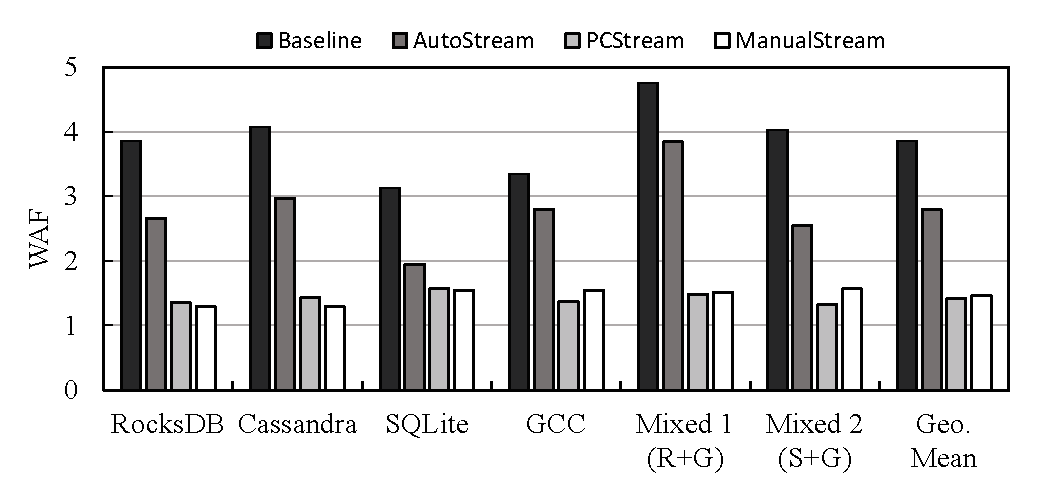
\includegraphics[width=1.\linewidth]{figure/pcstream/waf}
	\caption{A comparison of WAF under different schemes.}
	\label{fig:waf}
\end{figure}


%since the Manual scheme has static stream allocation.
%In Manual, once data types is mapped to the stream, the mapping is not changed 
%during runtime.
%For complex workloads which have large number of PCs such as mixed cases,
%it is difficult to expect data lifetimes in detail based on the data types.
%If the lifetime pattern is changed during runtime or the programmer choose
%second best stream mapping,
%Manual scheme lose the potential benefit in reducing WAf.
%However, the reclustering enables PCStream to adapt changing workload or find
%better stream mapping.
%The detailed analysis will be shown in the following subsections.
\subsection{Per-stream Lifetime Distribution Analysis}

To better understand the benefit of \textsf{\small PCStream} on the WAF
reduction, we measured per-stream lifetime distributions for the Mixed 1
scenario.  Fig.~\ref{fig:distribution} shows a box plot of data lifetimes from
the 25th to the 75th percentile.  As shown in Fig.~\ref{fig:distribution},
streams in both \textsf{\small PCStream} and \textsf{\small ManualStream} are
roughly categorized as two groups, $G1$ = $\{S_1$, $S_2$, $S_3$, $S_4$, $S_5\}$
and $G2$ = $\{S_6$, $S_7$, $S_8\}$, where $G1$ includes streams with short
lifetimes and small variances ({\it i.e.}, $S_1$, $S_2$, $S_3$, $S_4$, and $S_5$) and
$G2$ includes streams with large lifetimes and large variances ({\it i.e.}, $S_6$,
$S_7$, and $S_8$). The $S_0$ does not belong to any groups as it is assigned to
requests whose lifetimes are unknown.  Even though the variance in the $S_0$ is
wider than that in \textsf{\small ManualStream}, \textsf{\small PCStream}
showed similar per-stream distributions as \textsf{\small ManualStream}.  In
particular, for the streams in $G2$, \textsf{\small PCStream} exhibited smaller
variance than \textsf{\small ManualStream}, which means that \textsf{\small
PCStream} separates cold data from hot data more efficiently.  Since
\textsf{\small PCStream} moves long-lived data of a stream to its internal
stream, the variance of streams with large lifetimes tend to be smaller over
\textsf{\small ManualStream}.

\begin{figure}[t]
	\centering
	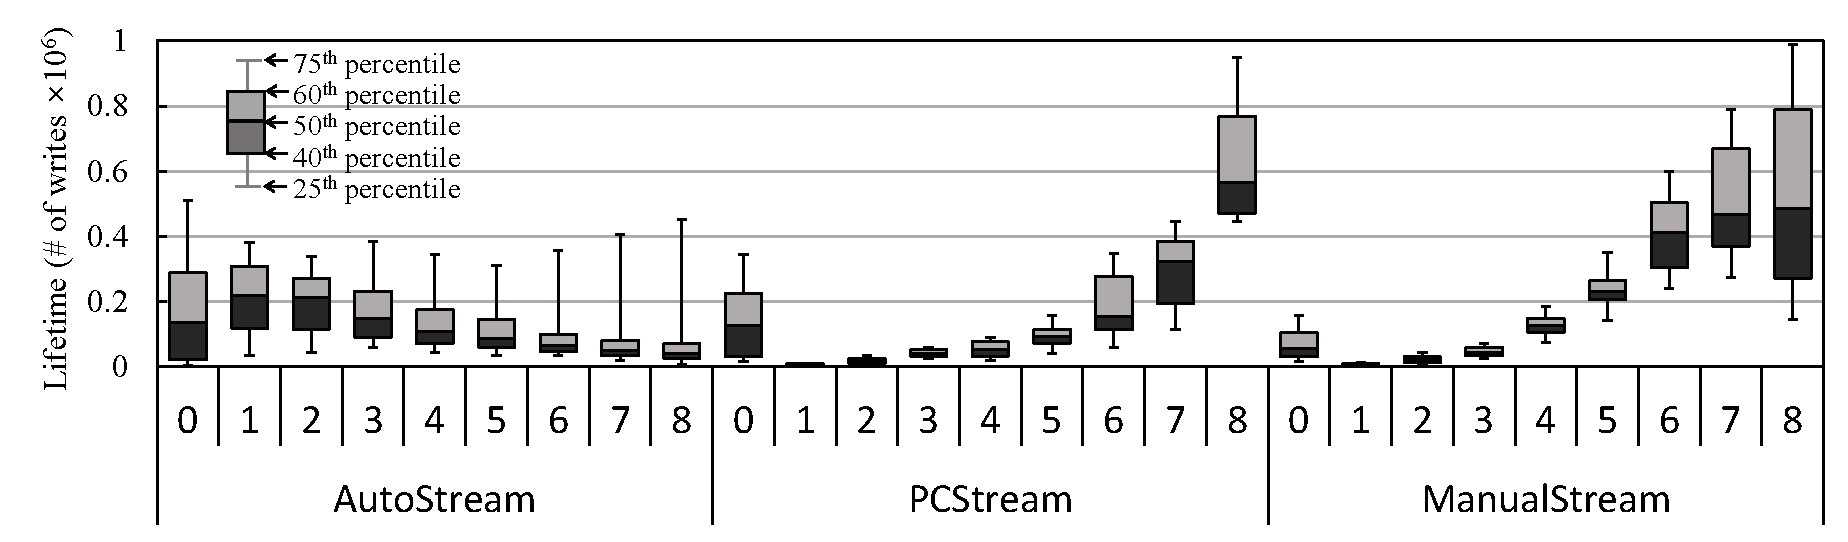
\includegraphics[width=1\linewidth]{figure/pcstream/distribution}
	\caption{A Comparison of per-stream lifetime distributions.}
	\label{fig:distribution}
\end{figure}


\textsf{\small AutoStream} was not able to achieve small per-stream variances
as shown in Fig.~\ref{fig:distribution} over \textsf{\small PCStream} and
\textsf{\small ManualStream}.  As shown in Fig.~\ref{fig:distribution}, all the
streams have large variances in \textsf{\small AutoStream} because hot data are
often mixed with cold data in the same stream.  Since the LBA-based data
separation technique of \textsf{\small AutoStream} does not work well with both
RocksDB and GCC, all the streams include hot data as well as cold data, thus
resulting in large lifetime variances. 

\subsection{Impact of Internal Streams}
\begin{figure}[t]
	\centering
	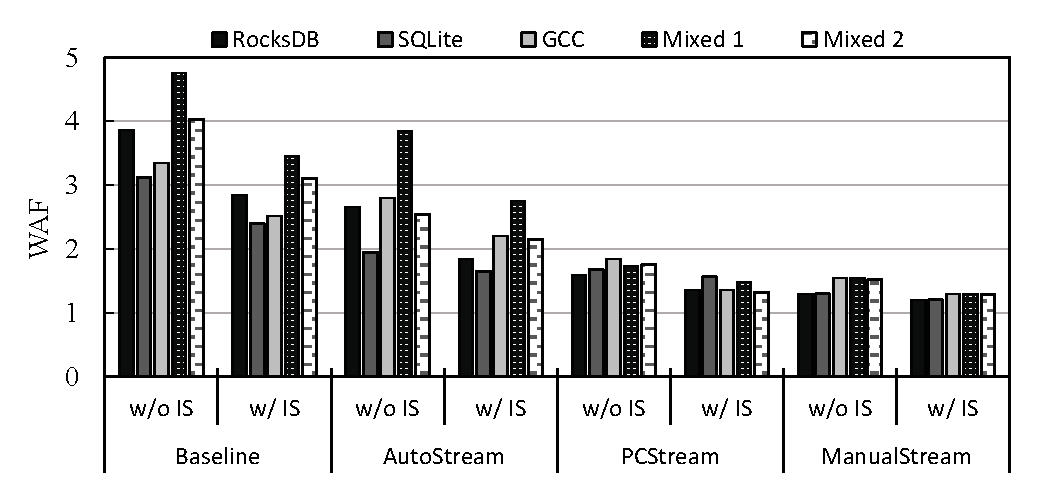
\includegraphics[width=1.\linewidth]{figure/pcstream/internal}
	\caption{The effect of internal streams on WAF.}
	\label{fig:internal}
\end{figure}

In order to understand the impact of internal streams on different stream
management techniques, we compared the two versions of each technique, one with
internal streams and the other without internal streams.  Since internal
streams are used only for GC, they can be combined with any
existing stream management techniques.  Fig.~\ref{fig:internal} shows WAF values
for five benchmarks with four techniques.  Overall, internal streams worked
efficiently across the four techniques evaluated.   When combined with
internal streams, \textsf{\small Baseline}, \textsf{\small AutoStream},
\textsf{\small PCStream} and \textsf{\small ManualStream} reduced the average
WAF by 25\%, 22\%, 17\%, and 12\%, respectively.  Since the quality of initial
stream allocations in \textsf{\small Baseline} and \textsf{\small AutoStream}
was relatively poor, their WAF improvement ratios with internal streams were
higher over \textsf{\small PCStream} and \textsf{\small ManualStream}.
Although internal streams were effective in separating short-lived data from
long-lived data in both \textsf{\small Baseline} and \textsf{\small
AutoStream}, the improvement from internal streams in these techniques are not
sufficient to outperform \textsf{\small PCStream} and \textsf{\small
ManualStream}.  Poor initial stream allocations, which keep putting both hot
and cold data to the same stream, unfortunately, offset a large portion of
benefits from internal streams.



\subsection{Impact of the PC Attribute Table}
As explained in Section~\ref{sec:PC_lf_mngm}, the PC attribute table is useful to maintain a
long-term history of applications' I/O behavior by exploiting the uniqueness of
a PC signature across different applications.   To evaluate the effect of the
PC attribute table on the efficiency of \textsf{\small PCStream}, we modified
the implementation of the PC attribute table so that the PC attribute table can
be selectively disabled on demands when a process terminates its execution.
For example, in the kernel compilation scenario with GCC, the PC attribute
table becomes empty after each kernel build is completed.  That is, the next
kernel build will start with no existing PC to stream mappings.


\begin{figure}[t]
	\centering
	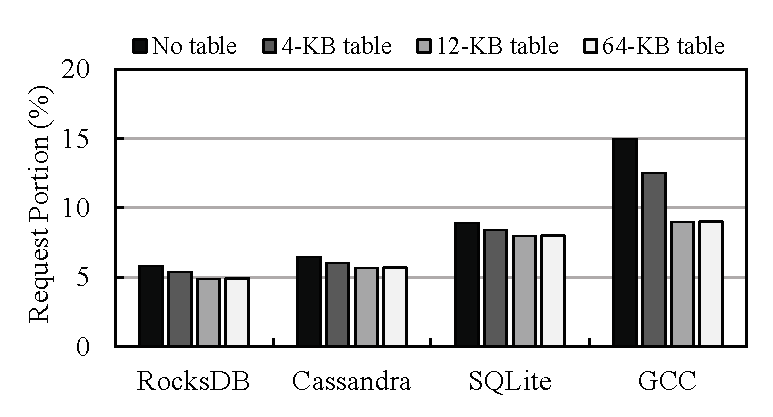
\includegraphics[width=1\linewidth]{figure/pcstream/pctable}
	%\caption{The effect of the PC attribute table on the default stream allocation.}
	\caption{The effect of the PC attribute table.}
	\label{fig:pctable}
\end{figure}

Fig.~\ref{fig:pctable} show how many requests are assigned to the default
$S_{0}$ stream over varying sizes of the PC attribute table.  Since $S_{0}$ is
used when no stream is assigned for an incoming write request, the higher the
ratio of requests assigned to $S_{0}$, the less effective the PC attribute
table.   As shown in Fig.~\ref{fig:pctable}, in RocksDB, Cassandra, and SQLite,
the PC attribute table did not affect much the ratio of writes on $S_{0}$.
This is because these programs run continuously for a long time while
performing the same dominant activities repeatedly.  Therefore, although the PC
attribute table is not maintained, they can quickly reconstruct it.  On the
other hand, the PC attribute table was effective for GCC, which frequently
creates and terminates multiple processes ({\it e.g.}, {\tt cc1}).  When no PC
attribute table was used, about 16\% of write requests were assigned to
$S_{0}$.  With the 4-KB PC attribute table, this ratio was reduced to 12\%.
With the 12-KB PC attribute table, only 9\% of write requests were assigned to
$S_{0}$.  This reduction in the $S_{0}$ allocation ratio reduced the WAF value
from 1.96 to 1.54.



\chapter{Fine-grained Deduplication Technique using Program Contexts} 
\label{chap:FineDedup}

\section{Overview}
As the price-per-byte of NAND flash memory is rapidly decreasing,
NAND flash-based solid-state drives (SSDs) are emerging as a viable high-performance storage solution
for laptops, desktop PCs and high-performance enterprise systems.
However, as NAND flash memory technology scales down to 20-nm and below~\cite{tlc}, storing data reliably in NAND flash memory
gets a key design challenge of NAND-based storage systems. 
%For example, the number of program/erase (P/E) cycles allowed for each block is significantly reduced in recent triple-level cell (TLC)
%NAND technology.
%While older 5x-nm single-level cell (SLC) NAND flash memory can support about 10 K P/E cycles, recent 2x-nm TLC NAND flash memory
%can barely support about 1 K P/E cycles~\cite{tlc}.
Particulary, the reduction in the number of P/E cycles of NAND flash memory seriously limits the overall lifetime of flash-based SSDs,
making it difficult for SSDs to be used in write-intensive applications.

In order to extend the lifetime of flash-based SSDs,
data deduplication techniques have been used in recent SSDs
because they are effective in reducing the amount of data written to flash memory by preventing duplicate data 
from being written again~\cite{caftl,value-locality}.
As a result, only non-duplicate data, i.e., unique data, are stored in SSDs, thus effectively decreasing the total amount of data written to
SSDs.
In most deduplication schemes proposed for SSDs,
the unit of data deduplication is the same as the flash page size which is usually 4 KB or 8 KB.
%Using a page as a deduplication unit seems to be reasonable 
%because the unit of a read or write operation of flash memory is also a page. 
However, this page-based deduplication technique misses many chances of eliminating duplicate data, especially
when two pages are \textit{almost} identical.
%For example, in our experimental analysis of an existing 4 KB page-based deduplication technique, we observed that
%up to 34\% mostly identical data.
%If the unit of deduplication were smaller than 4 KB, about 23\% more data could be identified as duplicate data.
Furthermore, it is expected that the effectiveness of the page-based deduplication technique would 
get even worse in future NAND flash memory as the page size of 
flash memory is expected to increase
to a bigger size such as 16 KB~\cite{16kpage}.

In this dissertation, 
we propose a fine-grained deduplication technique for flash-based SSDs, called \textit{FineDedup}.
The proposed FineDedup technique is different from other existing deduplication techniques
in that it increases the likelihood of finding duplicates
by using a finer deduplication unit
which is smaller than a single page (e.g., one fourth of a single page).
With a smaller deduplication unit,
many data segments within a page can be detected as a duplicate one, 
so the amount of data written to flash memory can be reduced regardless of a physical page size.

In order to effectively incorporate fine-grained deduplication into flash-based SSDs,
two key technical issues must be addressed properly.
First, fine-grained deduplication requires a larger memory space than a coarse-grained one 
because it needs to keep more metadata in memory to find small-size duplicate data.
Second, in fine-grained deduplication, 
unique data segments from partially duplicated pages can be scattered across several physical pages,
which may seriously degrade the overall read performance.
The proposed FineDedup technique is designed to take full advantage of fine-grained deduplication
with small memory overhead as well as a low read performance penalty.
Our evaluation results show that 
FineDedup prolongs the lifetime of SSDs by up to 24\% over page-based deduplication
while requiring a negligible memory space increase.
This improvement comes with a less than 5\% read performance penalty over page-based deduplication.

\section{Selective Deduplication using Program Contexts}
As analyzed in Section~\ref{sec:duplicateactivity}, data duplicate patterns and I/O activities seems to
have relationship. 
Particulary, some writes are known a priori
to be likely to be unique. Applications might generate
data that should not or cannot be deduplicated. For
example, some applications write random, compressed,
or encrypted data; others write complex formats (e.g.,
virtual disk images) with internal metadata that tends to
be unique.

Attempting to deduplicate unique writes wastes CPU
time on hash computation and I/O bandwidth on maintaining
the hash index. Unique hashes also increase the
index size, requiring more RAM space and bandwidth
for lookup, insertion, and garbage collection.

In summary, if program context can help to
know when it is unwise to deduplicate a write, we can optimize
its performance and reliability. We implemented
a selective deduplication based on the program context.

Since deduplication uses computational resources
and may increase latency, it should only be performed
when there is a potential benefit. The program context
hint instructs the device not to deduplicate a particular
writes. It has two use cases:
(1) unique data: there is no point in wasting resources
on deduplicating data that is unlikely to have duplicates,
such as short-lived data; (2) reliability: maintaining
multiple copies of certain writes may be necessary,
e.g., superblock replicas in many file systems.

\begin{figure}[t]
	\center
	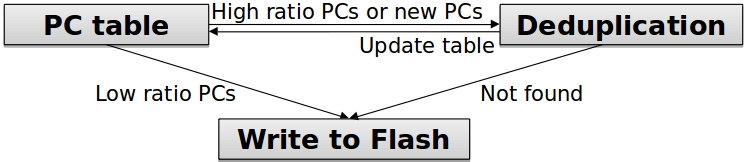
\includegraphics[scale=0.3]{figure/finededup/selectivededup}
	\caption{Diagram of selective deduplication.} % ok
	\label{fig:selectivededup}
\end{figure}

Figure~\ref{fig:selectivededup} shows a diagram of the proposed selective
deduplication technique. 
When a write request comes, it first query its PC value to the PC table which holds 
duplicate rate per PCs.
If the PC has high duplicate ratio or a new one, we apply deduplication on the request.
After fingerprinting and searching, the result is updated to the PC table.
If the PC has low duplicate ratio or there is no written data for a new PC,
we handle data as a normal reqeust.


\section{Exploiting Small Chunk Size }
\label{sec:finededup_motivation}

The write-requested page is identified whether the contents of the page have already been written and 
is written to flash memory only if there is no existing duplicate page. 
When a write-requested page is the exact duplicate of a previously written page, 
the requested page is not written to flash memory; 
only the corresponding entry for a mapping table (between the logical address and physical address) is updated. 
On the other hand, if there is no existing page duplicate in flash memory whose contents are the 
same as those of requested one, the requested page has to be written to flash memory. 
However, even for these unique pages, if their redundancy is checked at a sub-page level, 
say at a quarter of the page size, many sub-pages of these unique pages can be identified as redundant data. 
In existing techniques based on page-level deduplication, therefore, 
many duplicate data are written to flash memory even though the same data chunks have already been written.

In order to better understand the effect of fine-grained deduplication on the amount of identified duplicate data,
we analyzed how many more chunks can be identified as redundant 
when the chunk size gets smaller than a single page.
For our evaluation, we used four I/O traces, \texttt{RocksDB}, \texttt{GCC+cp}, \texttt{PC usage}, and \texttt{Package Tool} which are 
explained in Section~\ref{sec:finededup_experimentalresult}.
%collected from a desktop PC and a number of server systems used for a hardware synthesis, and a sensor data analysis.
In our evaluation, the page size was 4 KB and the chunk size was set to 1 KB.

\begin{figure}[t]
	\center
	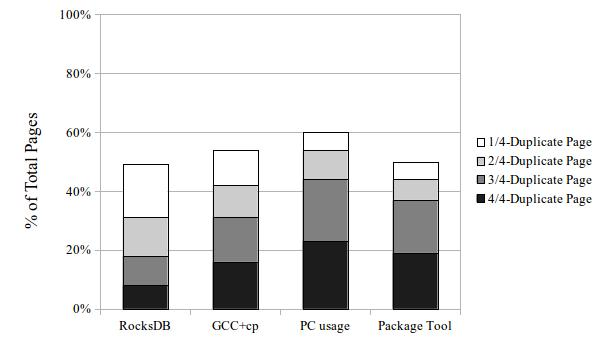
\includegraphics[scale=0.5]{figure/finededup/dupChunkperReq_}
	\caption{The percentage of pages according to their partial duplicate patterns.} % ok
	\label{fig:percentage}
\end{figure}

Fig.~\ref{fig:percentage} shows the percentage of the page writes from host, classified by their partial duplicate patterns.
We denote that a page is a n/4-duplicate page when n chunks of the page are duplicate chunks.
A 4/4-duplicate page is a duplicate page at the page level.
In the existing page-based deduplication, only 4/4-duplicate pages can be identified as a duplicate page.
As shown in Fig.~\ref{fig:percentage}, 4/4-duplicate pages account for only 8\% - 28\% of total requested pages.
%However, for partially duplicate pages where the number of duplicate chunks within a requested page is between 1 and 3,
For partially duplicate pages, i.e., 1/4-, 2/4- and 3/4-duplicate pages, the page-based deduplication technique is useless.
As shown in Fig.~\ref{fig:percentage},
pages with 1-3 duplicate chunks account for 14\% - 34\%.
This means that many duplicate data are unnecessarily written to flash memory
due to the large chunk size.
%when the size of a chunk is large.

\begin{figure}[t]
	\center
	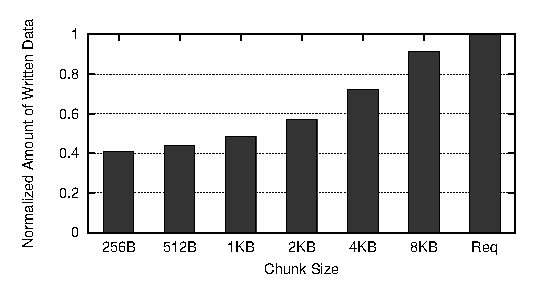
\includegraphics[scale=1]{figure/finededup/nonDuplicatedData_ChunkSize}
	\caption{The amount of written data under varying chunk sizes in \texttt{PC} workload.} % ok
	\label{fig:chunksize}
\end{figure}

We also investigated the amount of data that can be eliminated by data deduplication 
while varying the chunk size from 256 B to 8 KB.
As shown in Fig.~\ref{fig:chunksize}, 
when the chunk size is 1 KB, 
the amount of data written to flash memory is reduced by 33\% over when the chunk size is 4 KB.
In particular, when the size of a chunk is 8 KB (i.e., when the physical page size is assumed to be 8 KB),
only 10\% of requested data are eliminated by data deduplication.
This effectively shows that, as the size of a page increases,
the overall deduplication ratio, i.e., the percentage of identified duplicate writes, decreases significantly.
Since the physical page size of NAND flash memory is expected to increase as the semiconductor process is scaled down~\cite{tlc,16kpage},
it is expected that the deduplication ratio of the existing deduplication technique will be significantly 
decreased in near future.
In order to resolve this problem, the deduplication chunk size of deduplication techniques needs to be smaller than a page size.
As depicted in Fig.~\ref{fig:chunksize}, 
the deduplication ratio is saturated when the chunk size is 1 KB.
Thus, we use it as a default chunk size in the rest of this dissertation.



\section{Fine-Grained Deduplication}
\label{sec:finededup_finededup}
In order to effectively incorporate fine-grained deduplication into flash-based SSDs,
two key technical issues must be addressed properly.
First, fine-grained deduplication requires a larger memory space than a coarse-grained one 
because it needs to keep more metadata in memory to find small-size duplicate data.
Second, in fine-grained deduplication, 
unique data segments from partially duplicated pages can be scattered across several physical pages,
which may seriously degrade the overall read performance.
The proposed FineDedup technique is designed to take full advantage of fine-grained deduplication
with small memory overhead as well as a low read performance penalty.

In this section, we describe our proposed FineDedup technique in detail.
We first explain the overall architecture of FineDedup and 
describe how FineDedup handles read and write requests in Section~\ref{sec:finededup_architecture}.
In Section~\ref{sec:finededup_readoverheadmanagement} and ~\ref{sec:finededup_memoryoverheadmanagement}
we introduce a read performance penalty and memory overheads caused by FineDedup, respectively,
and explain how these problems can be resolved in FineDedup.

\subsection{Overall Architecture of FineDedup}
\label{sec:finededup_architecture}

Fig.~\ref{fig:overview} shows an overall architecture of FineDedup with its main components.
Upon the arrival of a write request,
FineDedup stores requested data temporarily in an on-device buffer,
which is managed by an LRU algorithm.
When the requested data are evicted from the buffer,
FineDedup divides the data into several chunks.
(Note that the chunk size is 1 KB in this work, 
but a different size of chunks can be used as well in FineDedup.)

For each chunk, FineDedup computes a fingerprint, using a collision-resistant hash function.
In this work, we use an MD6 hash function~\cite{md6}, which is one of the well-known cryptographic hash functions.
A fingerprint is used as a unique ID that represents the contents of a chunk.
FineDedup has to compute more fingerprints than the existing deduplication schemes
because of its small chunk size.
To reduce the hash calculation time,
FineDedup uses multiple hardware-assisted hash engines for parallel hash calculations. 
In our FPGA (ML605) implementation of the MD6 hash function, it took about 10 $\mu$s to compute a fingerprint using a hardware accelerator.
Considering a long write latency (e.g., 1.2 $m$s) of NAND flash memory,
the time overhead of computing fingerprints can be considered negligible.

After fingerprinting, 
each fingerprint is looked up in the dedup table
which maintains the fingerprints of the unique chunks previously written to flash memory.
Each entry of the dedup table is composed of a key-value pair, \{\textit{fingerprint}, \textit{location}\},
where the location indicates a physical address in which the unique chunk is stored.
If the same fingerprint is found,
it is not necessary to write the chunk data
because the same chunk is already stored in flash memory.
Instead, FineDedup updates the mapping table 
so that the corresponding mapping entry points to the unique chunk previously written.
Unlike existing page-based deduplication techniques,
FineDedup handles all the data in the unit of a chunk.
%For this reason, FineDedup must maintain a chunk-level mapping table,
%which is much larger than the existing page-level mapping table.
For this reason, FineDedup must maintain a chunk-level mapping table
that maps a logical chunk address to a physical chunk in flash memory.
Because of its finer mapping granularity,
the chunk-level mapping table is much larger than the existing page-level mapping table.
To reduce the memory space for maintaining the chunk-level mapping table,
FineDedup uses a hybrid mapping strategy,
which is described in Section~\ref{sec:finededup_memoryoverheadmanagement} in detail.

\begin{figure}[t]
	\center
	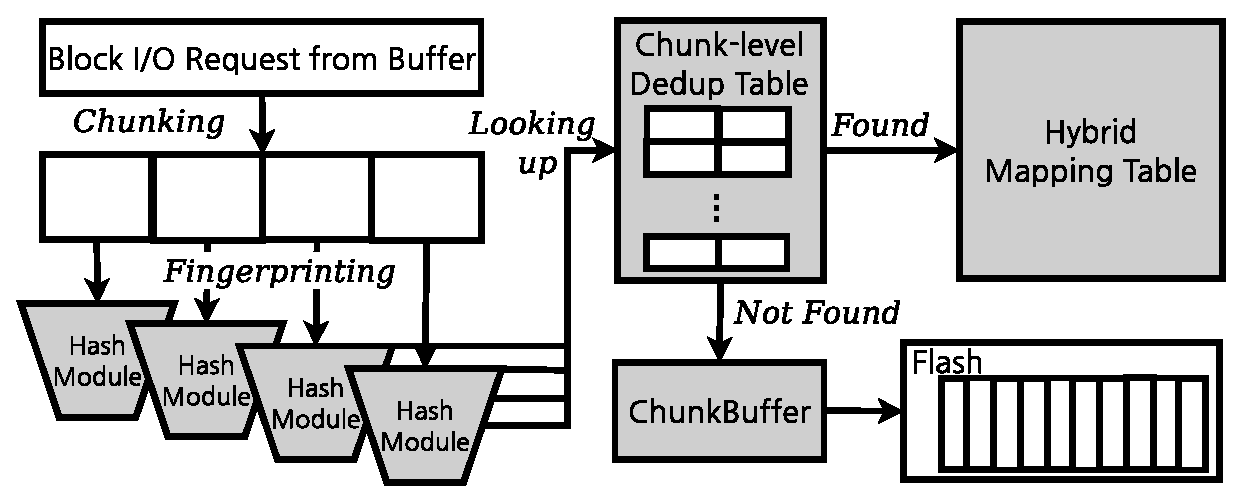
\includegraphics[scale=0.4]{figure/finededup/overview}
	\caption{An overview of the proposed FineDedup technique.} % ok
	\label{fig:overview}
\end{figure}

If there is no matched fingerprint in the dedup table,
FineDedup stores the chunk data in a \textit{chunk buffer} temporarily.
This temporary buffering is necessary 
because the unit of I/O operations of flash memory is a single page.
The chunk buffer stores the incoming chunk data until there are four chunks,
and evicts them to flash memory at once.
FineDedup then updates the mapping table 
so that the corresponding mapping entries indicate newly written chunks.
The new fingerprints of the evicted chunks are finally inserted into the dedup table with their physical location.

When a read request arrives,
FineDedup reads all the chunks that belong to the requested page from flash memory,
and then transfers the read data to the host system.
The physical addresses of the chunks can be obtained by consulting to the mapping table.
In FineDedup, four chunks in the same logical page can be scattered across different physical pages.
In that case, multiple read operations are required to form the original page data,
which in turn significantly increases the overall read response time.
We explain how FineDedup resolves this problem in the following subsection.

\subsection{Read Overhead Management}
\label{sec:finededup_readoverheadmanagement}

FineDedup effectively reduces the number of pages written to flash memory
by using a small-size chunk for deduplication,
but it incurs two types of additional overheads, i.e.,
a read performance overhead and a memory space overhead,
which are not observed in the existing deduplication techniques.
In this subsection, 
we first introduce why the read performance overhead occurs in FineDedup,
and then explain how FineDedup resolves this problem.
In the following subsection, 
we describe our memory space overhead reduction technique in detail.

The main cause of the read performance degradation is data fragmentation
which occurs when data chunks belonging to the same logical page are broken up into several physical pages.
Fig.~\ref{fig:readoverhead} illustrates why data fragmentation occurs in FineDedup.
There are two page write requests, \textit{Req 1} and \textit{Req 2}, in Fig.~\ref{fig:readoverhead}.
\textit{Req 1} consists of four chunks, `A', `B', `C', and `D', 
and \textit{Req 2} is also composed of four chunks, `E', `F', `G', and `H'.
Since `A' and `B' of \textit{Req 1} are duplicate chunks,
only `C' and `D' need to be written to flash memory.
%Thus, we can reduce writes for two chunks `A' and `B'.
Suppose that there is a read request for the page data written by \textit{Req 1}.
%after the chunks of \textit{Req1} are written to flash memory.
In that case, FineDedup has to read three pages, i.e., \textit{page 1}, \textit{page 2}, and \textit{page 3}, from flash memory
to form the requested data.
%to form the requested data of \textit{Req1}, incurring a significant read performance penalty.
The read performance penalty can also occur even when there are no duplicate chunks in the requested page.
For example, in Fig.~\ref{fig:readoverhead}, 
\textit{Req 2} has no duplicate chunks in flash memory,
thus all the chunks belonging to \textit{Req 2} being written to flash memory.
Because a single page write requires four data chunks, 
`E' and `F' of \textit{Req 2} are written to \textit{page 3} together with `C' and `D',
and `G' and `H' will be written to \textit{page 4} with other data chunks, as shown in Fig.~\ref{fig:readoverhead}.
Thus, when the data written by \textit{Req 2} are read later, 
both \textit{page 3} and \textit{page 4} must be read from flash memory.

\begin{figure}[t]
	\center
	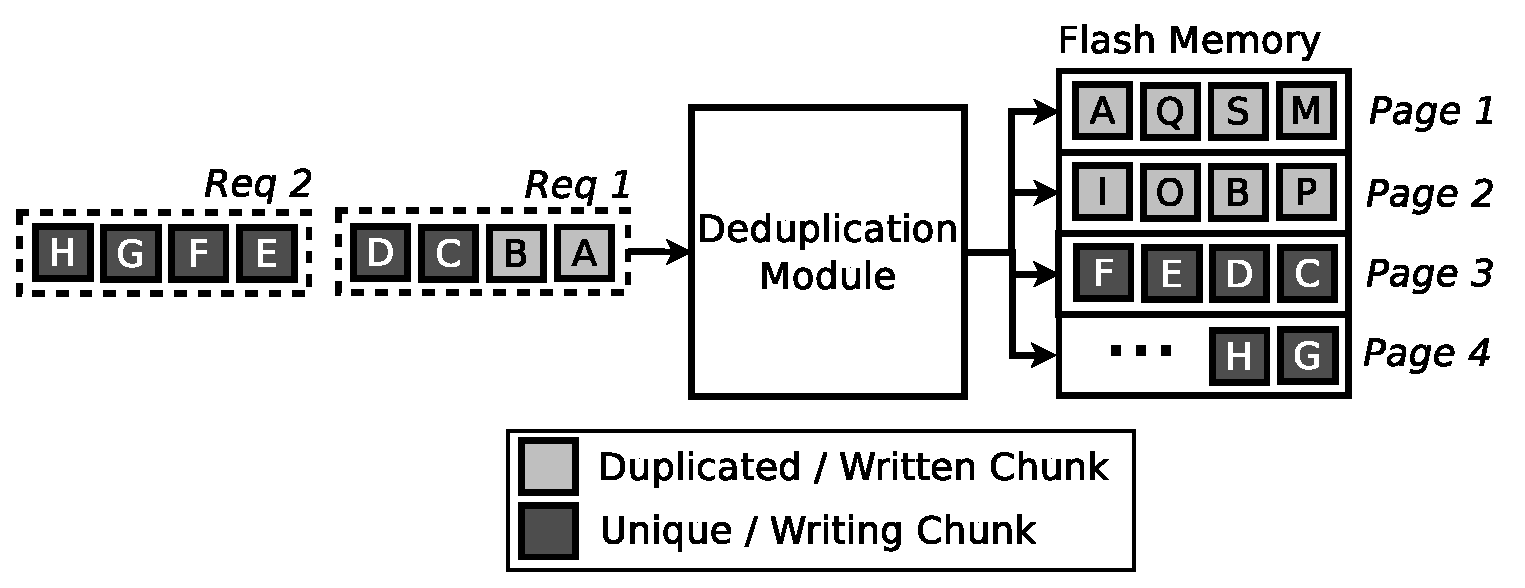
\includegraphics[scale=0.4]{figure/finededup/readoverhead}
	\caption{Data fragmentation caused by FineDedup.} % ok
	\label{fig:readoverhead}
\end{figure}


One of the feasible approaches that mitigate the read performance overhead is to employ a chunk read buffer.
In our observation, 
the access frequencies of unique chunks are greatly skewed;
that is, a small number of popular chunks account for a large fraction of the total accesses to unique chunks in flash memory.
For example, according to our analysis under real-world workloads, 
top 10\% of the unique chunks serve more than 70\% of the total data read by a host system.
By keeping frequently accessed chunks in a chunk read buffer,
therefore, FineDedup can reduce a large number of page read operations sent to flash memory.

\begin{figure}[t]
	\center
	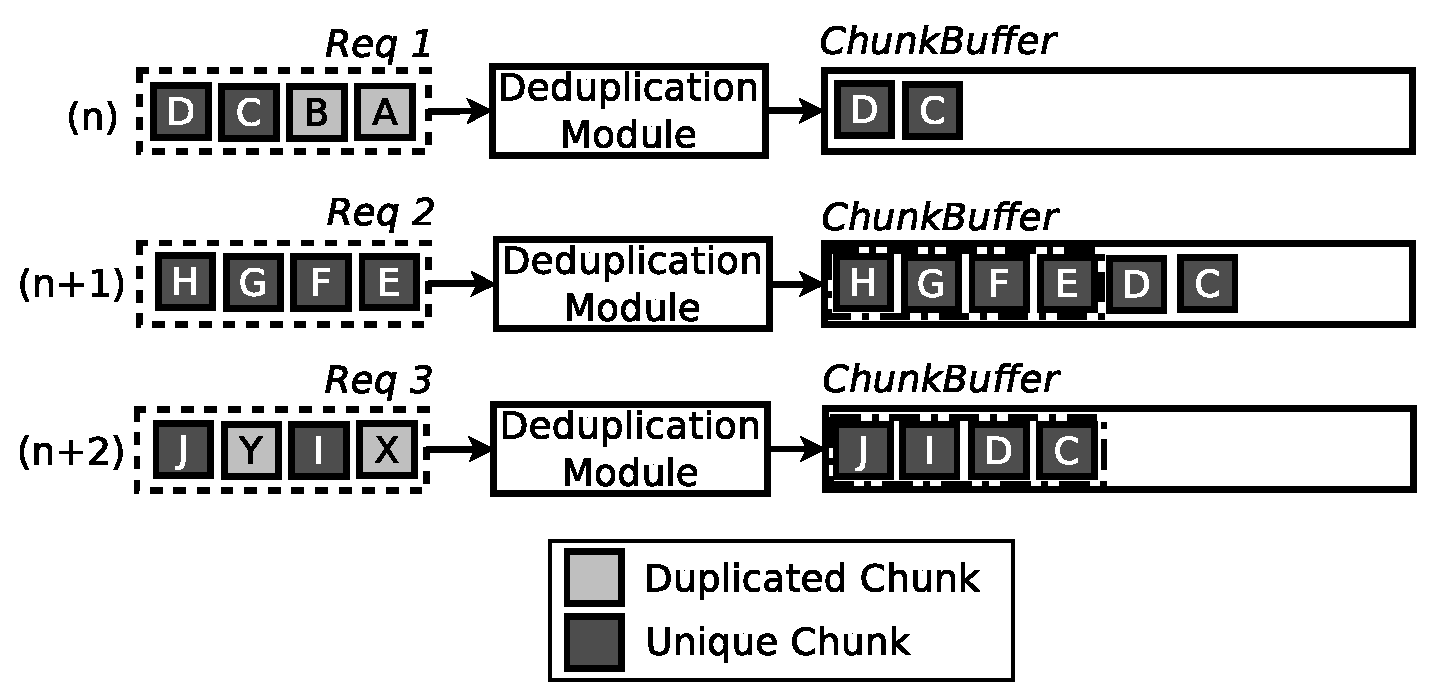
\includegraphics[scale=0.4]{figure/finededup/chunkbuffer}
	\caption{A packing scheme in the \textit{chunk buffer}.} % ok
	\label{fig:chunkbuffer}
\end{figure}

On the other hands, we have observed that about 39\% of read requests to unique pages actually requires two page read operations.
In order to further reduce this read performance penalty,
FineDedup uses a chunk packing scheme.
The key idea of this scheme is to
group chunks belonging to the same logical page in a chunk buffer and 
then write them to the same physical page together.
Fig.~\ref{fig:chunkbuffer} shows an example of our chunk packing scheme
when three page write requests, \textit{Req 1}, \textit{Req 2}, and \textit{Req 3}, are consecutively issued from a host system.
\textit{Req 1} contains two duplicate chunks `A' and `B' and two unique chunks `C' and `D'.
As expected, only `C' and `D' out of four chunks are sent to the chunk buffer.
The next request \textit{Req 2} does not have any duplicate chunks,
so all of them are moved to the chunk buffer.
As depicted in Fig.~\ref{fig:chunkbuffer},
the chunks `E', `F', `G', and `H' belong to the same logical page and form single page data.
Thus, FineDedup writes them to flash memory together,
leaving the chunks `C' and `D' in the chunk buffer.
When \textit{Req 3} is issued with two more unique chunks `I' and `J', 
`C' and `D' along with `I' and `J' are written to flash memory.
All those chunks can be written to the same physical page together
because every chunk of each request is not broken up into two pages.

Note that the main objective of this scheme is to prevent chunks of a unique request to be scattered across multiple pages 
avoiding unnecessary data fragmentation.
In order to directly insert a incoming unique request to chunk buffer,
page-sized free space is managed to be always available in the buffer.
When there is no free space for the next request and no suitable chunks of requests to form a single page,
the chunks of a partially duplicate request is broken up into two pages.
Most partially duplicated requests, however, are 3/4-Duplicate pages as shown in Fig.~\ref{fig:percentage}, which means 
there are many requests of one unique chunk in the chunk buffer.
Therefore, we can expect that most requests will be written to the same page even when the size of the chunk buffer is not large 
since it is not quite difficult to find an appropriate chunk to fit a flash page.
In the above example, if we assume the chunk buffer can contain 8 chunks and \textit{Req 3} has three unique chunks,
only two chunks of \textit{Req 3} will be written along with existing chunks, `C' and `D', leaving the other chunk in chunk buffer.
A large chunk buffer provides more chance to avoid the request scattering.


%%%%% NEED TO BE EXPLAINED!!! POWER FAILURE 시 partial chunks 'C', 'D' 가 power-off recovery 될 수 있음. => reliability 관리  %%%
Remaining data in the chunk buffer could be lost when a power failure occurs.
Recent enterprise SSDs, such as SM825 model manufactured by Samsung, have a large SDRAM cache (e.g., 256 - 512 MB) and use it as a device buffer.
Moreover, they support internal cache power protection through the use of capacitors to flush out information in DRAM to flash memory 
at the event of power failure~\cite{sm825}.
In order to keep the reliability in FineDedup, the remaining data in the chunk buffer can be stored to flash memory 
during power protection procedure as well as the mapping information of the written page.
In conclusion for chunk buffer design, there is a trade-off between potential read performance 
and reliability depending on the chunk buffer size.
The size of the chunk buffer, hence, should be determined according to the characteristics of workloads.

\subsection{Memory Overhead Management}
\label{sec:finededup_memoryoverheadmanagement}

As mentioned in Section~\ref{sec:finededup_architecture},
FineDedup handles requested data in the unit of a chunk.
Therefore, FineDedup must maintain a chunk-level mapping table
that maps a logical chunk address to a physical chunk address in flash memory.
Since the size of a chunk is smaller than that of a page,
a chunk-level mapping table is much larger than the page-level mapping table.
For example, suppose that the page size is 4 KB and the chunk size is 1 KB.
In that case, the size of a chunk-level mapping table is four times larger than that of a page-level mapping table.

In order to reduce the amount of memory space required for a mapping table,
FineDedup employs a hybrid mapping table
which is composed of two types of mapping tables:
a page-level mapping table and a chunk-level mapping table.
As depicted in Fig.~\ref{fig:percentage}, 
duplicate pages and unique pages still account for a considerable proportion of the total written pages.
%for writing by a host system.
For these pages, the page-level mapping table is more appropriate 
because they can be directly mapped to corresponding pages in flash memory.
The chunk-level mapping table is required only for partially duplicate pages.

\begin{figure}[t]
	\center
	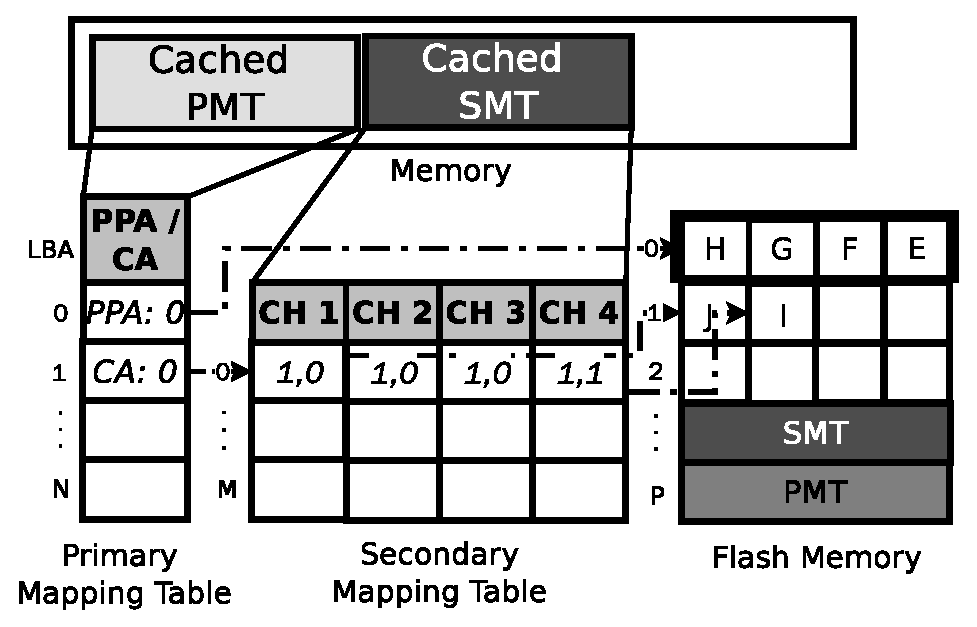
\includegraphics[scale=0.5]{figure/finededup/hybridmapping_1}
	\caption{An overview of the demand-based hybrid mapping table.} % ok
	\label{fig:hybridmapping}
\end{figure}


Fig.~\ref{fig:hybridmapping} shows the overall architecture of the hybrid mapping table used in FineDedup.
The primary mapping table (PMT) is maintained in the page level 
while the secondary mapping table (SMT) is maintained in the chunk level.
The entry of the PMT is either a physical page address (PPA in Fig.~\ref{fig:hybridmapping}) in flash memory or 
an index of the SMT (chunk address (CA) in Fig.~\ref{fig:hybridmapping}). 

%%%%%
%만약 request의 mapping 이 chunk 수준으로 관리될 필요가 없으면, 즉, unique page or fully duplicated page,  
If the chunk-level mapping is not necessary for a requested page, for example, unique page or duplicate page,
the corresponding entry of the PMT directly points to the physical address of the 
newly written page or existing unique page in flash memory, respectively.
%%%%%
%If the requested page is a duplicate one, 
%the corresponding entry of the primary mapping table directly points to the physical address of the existing unique page 
%in flash memory.
%Similarly, if the requested page is unique one, the corresponding entry of the primary mapping table is 
%updated to point to the newly written unique page.
%%%%
On the other hand, if a partially duplicate page is requested for writing, 
FineDedup allocates a new entry in the SMT.
As depicted in Fig.~\ref{fig:hybridmapping},
each entry of SMT is composed of four fields, each of which points to the physical chunk address 
in flash memory.
FineDedup then updates the new entry so that each field points to the physical chunk address.
The corresponding entry of the PMT indicates the newly allocated entry of the SMT.

Using the hybrid mapping table, 
FineDedup can reduce the amount of memory space for keeping a mapping table.
However, the problem of this hybrid mapping approach is that 
the size of a mapping table can greatly vary according to the characteristics of workloads.
For example, if some workloads have many partially duplicate pages, 
the size of the SMT gets too big.
On the other hand, if workloads mostly have unique pages or duplicate pages, 
the it can be very small.
Thus, the hybrid mapping table cannot be directly adopted in real SSD devices whose DRAM size is usually fixed.
To overcome such a limitation, 
FineDedup adopts a demand-based mapping strategy in which
the entire chunk-level mapping table is stored in flash memory
while caching only a fixed number of popular entries in DRAM memory.
The \textit{Cached PMT} and \textit{Cached SMT} in Fig.~\ref{fig:hybridmapping} represents the cached versions of the
PMT and SMT, respectively.

It has been known that the demand-based mapping requires extra page read and write operations~\cite{dftl}.
For instance,
if a mapping entry for a chunk to be read is not found in the in-memory mapping table,
that entry must be read from flash memory while evicting a victim entry to flash memory.
The temporal locality present in workload, however, helps keep the number of extra operations small.
The mapping information of requests issued in similar times will be stored in the same flash page.
Once a mapping page is loaded in memory, hence,
most requests issued in similar times are serviced from the mappings in memory.

\section{Experimental Results}
\label{sec:finededup_experimentalresult}

%In this section, 
%we first describe our experimental settings and explain the benchmarks used for our evaluation in detail.
%We then assess the effect of the proposed FineDedup technique on the SSD lifetime.
%Finally, we analyze the read performance penalty and the memory overhead caused by FineDedup.
%{\color{blue}We then analyze the benefit of the proposed FineDedup technique over the existing deduplication technique 
%in terms of the SSD lifetime and overheads such as the additional read operation and the required memory size.}


In order to evaluate the effectiveness of FineDedup, 
we performed our experiments using a trace-driven simulator with the I/O traces collected under various applications.
The trace-driven simulator modeled the basic operations of NAND flash memory, 
such as page read, page write and block erase operations,
and included several flash firmware algorithms, 
such as garbage collection and wear-leveling.
The proposed FineDedup technique and the existing deduplication techniques were also implemented in our simulator.

For trace collection, 
we modified the Linux kernel 2.6.32 and collected I/O traces at the level of a block device driver.
All the I/O traces include detailed information about the I/O commands sent to a storage device
(e.g., the type of requests, logical block addresses (LBA), the size of requests, etc.) 
as well as the contents of the data sent to or read from a storage device.
We recorded I/O traces while running various real-world applications.
The detailed descriptions of these I/O traces are summarized in Table~\ref{tab:traces}.

\begin{table}[t]
	\renewcommand{\tabcolsep}{1.4mm} 
	\centering
	\begin{tabular}{c|c|c|c}
		\hline
		\multirow{2}{*}{Trace} 		& \multirow{2}{*}{Description} 		& Amount of 	& Amount of \\
							   		& 			 				  		& Writes 		& Reads \\
		\hline
		\hline
		\multirow{2}{*}{\texttt{RocksDB}} 		& Benchmarking on the  & \multirow{2}{*}{3.1 GB} 	& \multirow{2}{*}{810 MB} \\
									   	   	    & Key-value store  		& 						 	& 						  \\
		\hline
		\multirow{2}{*}{\texttt{GCC+cp}}    	& Developing 		& \multirow{2}{*}{2.6 GB} 	& \multirow{2}{*}{66 MB} \\
											   	& Kernel modules  		& 							& 					   \\

		\hline
		\multirow{2}{*}{\texttt{PC usage}} 	   	& Web surfing, emailing and & \multirow{2}{*}{2.5 GB} 	& \multirow{2}{*}{70 MB} \\
											   	& editing document, etc. &   						& 						  \\

		\hline
		\multirow{2}{*}{\texttt{Package Tool}} 	 & Installing \& upgrading & \multirow{2}{*}{4.9 GB} 	& \multirow{2}{*}{119 MB} \\
										   	 & software packages			& 						   	& 					   \\
		\hline
	\end{tabular}
	\caption{A summary of traces used for experimental evaluations.}
	\label{tab:traces}
\end{table}


\subsection{Effectiveness of FineDedup}

\begin{figure}[t]
	\center
	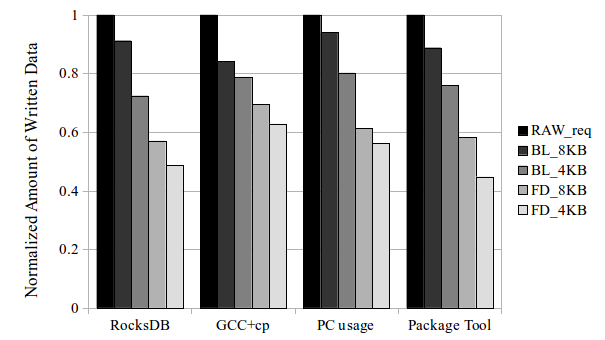
\includegraphics[scale=0.6]{figure/finededup/dataReduction_Chunksize_less_}
	\caption{The amount of written data under various schemes.} % ok
	\label{fig:reducedData}
\end{figure}


Fig.~\ref{fig:reducedData} shows the amount of data written to flash memory by FineDedup over the existing scheme.
The results shown in Fig.~\ref{fig:reducedData} are normalized to \textit{RAW\_req},
which represents the total amount of data written to flash memory without data deduplication.
We assume the page-based deduplication technique as a baseline case.
The baseline is denoted by \textit{BL\_4KB} for a 4 KB flash page and \textit{BL\_8KB} for a 8 KB flash page.
Our FineDedup technique is denoted by \textit{FD\_4KB} and \textit{FD\_8KB} for a 4 KB flash page and 
a 8 KB flash page, respectively.
The chunk size in FineDedup is set to 1 KB for a 4 KB flash page and 2 KB for a 8 KB flash page.

As we can see in Fig.~\ref{fig:reducedData}, 
the effectiveness of deduplication techniques is highly workload-dependent. 
The amount of data eliminated by the deduplication technique notably increases 
when FineDedup is applied in most of the traces except \texttt{M-media}.
%as the chunk size decreases in three traces, i.e., \texttt{PC}, \texttt{Sensor}, and \texttt{Synth}. 
When we set the chunk size to one fourth of the flash page size, 
FineDedup removes on average 16\% more duplicate data 
over \textit{BL\_4KB} for a 4 KB flash page.
For a 8 KB flash page, 
it removes more duplicate data, on average by 23\% over the existing technique.
For \texttt{RocksDB}, FineDedup saves 37\% flash writes over \textit{BL\_8K}.
As expected, the benefit of FineDedup mainly derives from the decreased chunk size 
because it increases the probability of finding and eliminating duplicate data.
Especially, \texttt{RocksDB} trace shows a large number of write requests with little different data during
compaction, so FineDedup can effectively 
identify unchanged data as duplicate while existing deduplication technique regards as unique data.

\subsection{Read Overhead Evaluation}
\label{sec:finededup_readoverheadevaluation}

\begin{figure}[t]
	\center
	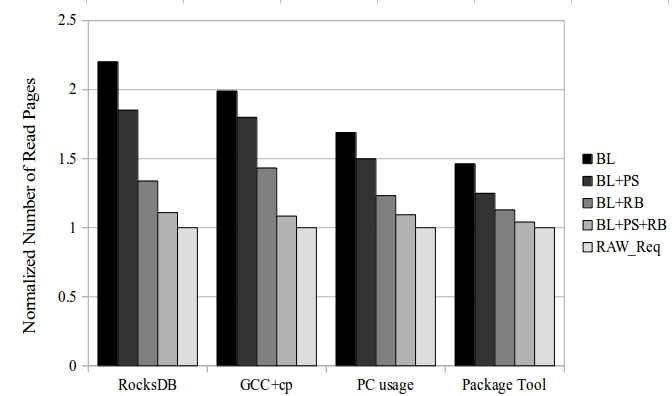
\includegraphics[scale=0.4]{figure/finededup/increasedPageRead_}
	\caption{The number of page read operations.} % ok
	\label{fig:pageread}
\end{figure}

As explained in Section~\ref{sec:finededup_readoverheadmanagement}, 
%subpage chunking in FineDedup increases the number of page read operations. 
fine-grained chunking in FineDedup increases the number of page read operations. 
%In FineDedup, we have have proposed the optimization techniques, such as the packing scheme and the chunk read buffer,
%to reduce additional page read operations.
Fig.~\ref{fig:pageread} shows the normalized number of page read operations compared with the number of read requests
in the workloads.
\textit{RAW\_Req} indicates the number of original page read requests and \textit{BL} refers to the number of page
read operations of the baseline FineDedup without employing proposed optimization schemes. 
\textit{BL+PS}, \textit{BL+RB} and \textit{BL+PS+RB} indicate the number of page reads of FineDedup with the proposed
packing scheme, the chunk read buffer, and both, respectively. 
The size of the chunk read buffer was set to 8 MB and the chunk buffer size was set to 200 KB.

As shown in Fig.~\ref{fig:pageread}, employing the chunk read buffer is more effective than the packing scheme 
for reducing additional page read operations in most workloads. This is because the packing scheme is only
effective for the requests containing no duplicate chunks whereas the chunk read buffer can absorb most of the read requests 
to frequently accessed chunks.
FineDedup with both the packing scheme and chunk read buffer incurs on average less than 5\% of additional read operations
over the existing deduplication technique.

\subsection{Memory Overhead Evaluation}
\label{sec:finededup_memoryoverheadevaluation}

As explained in Section~\ref{sec:finededup_memoryoverheadmanagement},
chunk level mapping table requires large memory space to handle partially duplicate pages.
In FineDedup, we have proposed 
the demand-based hybrid mapping table to reduce the required memory size for a mapping table without performance degradations.
In Fig.~\ref{fig:mappingoverhead}, the effectiveness of the proposed mapping table is evaluated in terms of the hit ratio and 
the amount of additional written data with various memory sizes for the cache.
Since the PMT of the hybrid mapping table in FineDeup is the same approach as the DFTL~\cite{dftl}, which is a well-known 
demand-based scheme to exploit the page-level mapping,
the overhead of PMT can be estimated from the overhead of DFTL.
Thus, in order to focus on the overhead of the SMT, we assume that DFTL is employed as the baseline mapping scheme in our evaluation.

\begin{figure}[t]
	\center
	\subfloat[Hit ratio of SMT cache]{\label{fig:mappingcachehit}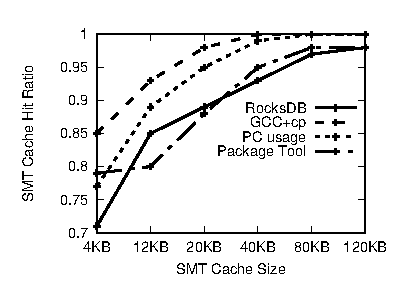
\includegraphics[scale=0.8]{figure/finededup/mappingcachehit_}}
	\subfloat[Extra data written due to SMT cache evictions]{\label{fig:mappingeviction}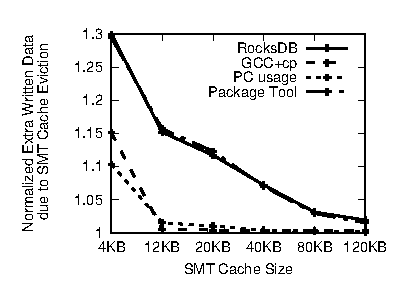
\includegraphics[scale=0.8]{figure/finededup/mappingeviction_}}
	\caption{The effectiveness of the demand-based hybrid mapping table in FineDedup with various cache sizes.}
	\label{fig:mappingoverhead}
\end{figure}

Fig.~\ref{fig:mappingoverhead}(a) shows the hit ratio of the cached SMT. 
With a 120 KB cache, more than 95\% of the mapping table accesses are absorbed.
In addition, Fig.~\ref{fig:mappingoverhead}(b) shows extra written data caused by the evicted page entries 
from the SMT cache.
Since mapping table accesses occur in the middle of read/write operations, it is important to reduce the 
amount of written data from evicted page entries in terms of read/write performance.
Similar to the hit ratio, the overhead by the eviction becomes almost negligible 
when the cache size is set to 120 KB under most workloads.
As a result, FineDedup does not incur a significant memory overhead 
even when the fine-grained chunking method is not effective.



\begin{comment}
\subsection{Evaluation of the Effectiveness of Cached Mapping Table for Mixed Workloads}

\begin{figure}[t]
	\center
	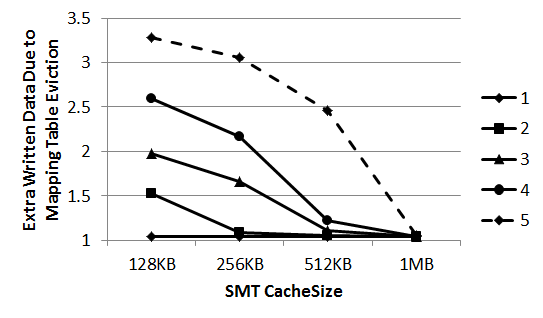
\includegraphics[scale=0.45]{figure/finededup/evicteddata_result.png}
	\caption{The amount of extra written data due to mapping table eviction for the mixed workload.} % ok
	\label{fig:eviction_mixed}
\end{figure}

The effectiveness of the cached mapping table is evaluated for mixed workloads. 
Fig.~\ref{fig:eviction_mixed} shows the normalized amount of additionally written data due to the 
mapping table eviction. 
The mixed traces are composed by accumulating individual traces in the order of 
\texttt{PC}, \texttt{Synth}, \texttt{Sensor}, \texttt{Install}, and \texttt{Update}. 
For example, mixed workload 4 is composed with \texttt{PC}, \texttt{Synth}, \texttt{Sensor}, and \texttt{Install}.
Although, the cached mapping table is not effective as the number of traces is increased, 
the performance degradation rate is smaller than the number of workload increasing rate. 
Moreover, mapping table caching will be effective when the caching memory is big enough to contain 
the working set of each trace. 
In the evaluation, the required memory space for the cached mapping table is about 1 MB for the mixed workload. 
Considering that commercial SSDs have hundreds of GBs of DRAM, the memory overhead of a few MB is not large.


\subsection{Evaluation of the Effectiveness of the Chunk Read Buffer}
\begin{figure}[t]
	\center
	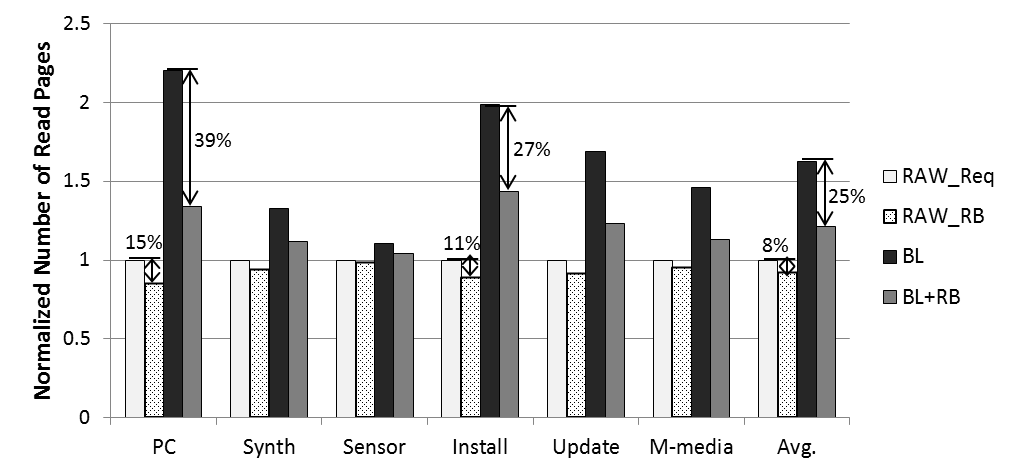
\includegraphics[scale=0.65]{figure/finededup/readbuffer_result.png}
	\caption{The number of page reads with and without read buffer.} % ok
	\label{fig:readbuffer}
\end{figure}

The effectiveness of the chunk read buffer between the baseline policy and FineDedup is evaluated. 
Fig.~\ref{fig:readbuffer} shows the amount of page reads for the baseline policy and FineDedup 
with and without the read buffer. 
The read buffer absorbs about 8\% read requests of \textit{RAW\_req}, whereas the read requests are 
reduced by about 25\% with the read buffer for FineDedup on average. 
Based on the analysis, the higher effectiveness of the read buffer in FineDedup is 
because of the increased memory utilization by deduplication. 
The read buffer in the baseline policy can absorb read requests for pages that have already been read. 
Chunk read buffer in FineDedup, however, can also absorb the read requests for deduplicated pages pointed 
by the hybrid mapping table. 
Therefore, with the same read buffer size, more read requests can be absorbed in FineDedup.


\subsection{Sensitivity Study on Chunk Read Buffer Size}
In addition to the evaluation of read overhead management shown in Section~\ref{sec:finededup_readoverheadevaluation},
we have evaluated that how the size of the chunk read buffer affects the number of read operations.
Fig.~\ref{fig:buffersize} shows the normalized number of read operations compared with the number
of read requests in the workloads while varying the buffer size from 8 KB to 32 MB.
The LRU scheme is used to be a replacement scheme in the chunk read buffer.
The chunk buffer is not used in this evaluation in order to focus only on the chunk read buffer.
When the buffer size gets larger, the number of read operations decreases.

\begin{figure}[t]
	\center
	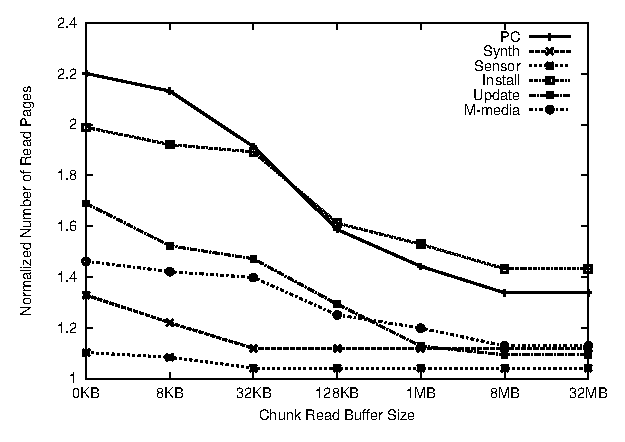
\includegraphics[scale=0.8]{figure/finededup/buffersize}
	\caption{The number of page read operations under varying chunk read buffer sizes.} % ok
	\label{fig:buffersize}
\end{figure}

As explained in Section~\ref{sec:finededup_readoverheadmanagement}, the access frequencies of unique chunks are greatly skewed.
Thus, it is important for read performance to keep those hot chunks in the chunk read buffer.
As shown in Fig.~\ref{fig:buffersize}, the chunk read buffer can absorb most read requests 
except for \texttt{PC} and \texttt{Install} traces.
In the \texttt{PC} and \texttt{Install} traces, 
the skewness of unique read accesses to hot chunks was significantly lower than other traces, thus
limiting the effectiveness of the chunk read buffer.
Since the effectiveness of the chunk read buffer diminishes as its size increases more than 8 MB,
in our experiments in Section~\ref{sec:finededup_readoverheadevaluation}, a 8 MB chunk read buffer was used.

\subsection{Sensitivity Study on Chunk Buffer Size}
\begin{figure}[t]
	\center
	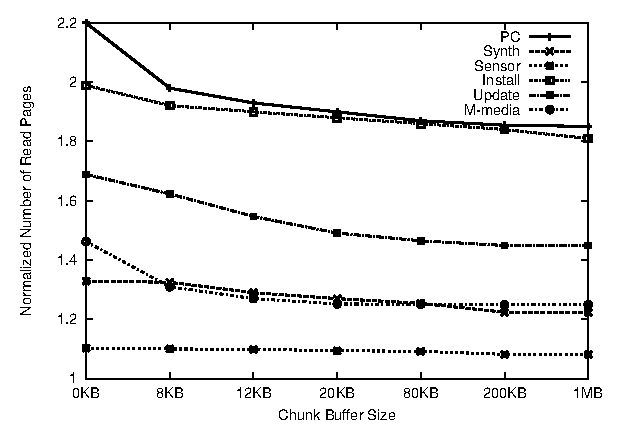
\includegraphics[scale=0.8]{figure/finededup/chunkbuffersize}
	\caption{The number of page read operations under varying chunk buffer sizes.} % ok
	\label{fig:chunkbuffersize}
\end{figure}


We have also evaluated that how the size of chunk buffer affects the number of read operations.
As explained in Section~\ref{sec:finededup_readoverheadmanagement},
the chunk buffer separates chunks of unique requests and chunks of partially duplicate requests.
Moreover, it also tries not to split chunks of partially duplicate requests into multiple pages.
Thus, a larger chunk buffer can reduce more potential extra read operations by preventing chunk splits.
Fig.~\ref{fig:chunkbuffersize} shows the normalized number of read operations compared with the number of read requests
in the workloads while varying the chunk buffer size from 8 KB to 1 MB.
For this evaluation, the chunk read buffer is not used to focus only on the chunk buffer.

As shown in Fig.~\ref{fig:chunkbuffersize}, the number of read operations does not decrease much as the chunk buffer size increases.
Since most partially duplicated requests in our traces is 3/4-Duplicate pages as explained
in Section~\ref{sec:finededup_readoverheadmanagement}, 
it is not difficult to find an appropriate chunk to fit a single flash page.
As shown in Fig.~\ref{fig:chunkbuffersize}, however, the benefit of chunk buffer is rather limited.
For example, there is no significant saving in the number of read pages for a chunk buffer larger than 200 KB. 
(In our experiment in Section~\ref{sec:finededup_readoverheadevaluation}, we used a 200-KB chunk buffer.)

	\end{comment}


\chapter{Conclusions}
\label{chap:Conclusions}

\section{Summary and Conclusions}
The cost-per-bit of NAND flash-based solid-state drives (i.e., SSDs) has 
steadily improved through uninterrupted semiconductor process scaling and 
multi-leveling so that they are how widely employed in not only mobile embedded 
systems but also personal computing systems.
However, the limited lifetime of NAND flash memory, as a side effect of recent 
advanced device technologies, is emerging as one of the major concerns for 
recent high-performance SSDs, especially for datacenter applications.

In this dissertation, we proposed several system-level techniques that improve
the lifetime of NAND flash-based storage devices. We first presented
data separation technique, called PCStream, for multi-streamed SSDs.
Unlike existing stream management techniques, \textsf{\small PCStream} fully automates 
the process of mapping data to a stream based on PCs, 
which work well for append-only workloads as well as update workloads.  
By exploiting an observation that most PCs are distinguishable from each other 
in their lifetime characteristics, \textsf{\small PCStream} allocates each PC to a different stream.  
When a PC has a large variance in their lifetimes, \textsf{\small PCStream} refines its stream allocation 
during garbage collection and moves the long-lived data of the current stream to its substream.  

Next, 
we propose a fine-grained deduplication technique for flash-based SSDs, called FineDedup.
By using a fine-grained deduplication unit,
the proposed FineDedup technique increases the amount of data eliminated 
by data deduplication by up to 37\% over the existing page-based deduplication technique,
extending the SSD lifetime by the same amount.
FineDedup inevitably increases the overall read response time because of data fragmentation.
By employing a chunk read buffer and a chunk packing scheme,
however, the read performance overhead is limited to less than 5\% 
in comparison with the existing deduplication technique.
To reduce the memory space required for a chunk-level mapping table,
FineDedup adopts a hybrid mapping scheme.
Our evaluation results show that 
FineDedup is effective in improving the SSD lifetime,
requiring only about 10 MBs of more memory space in total.

\section{Future Work}
\subsection{Improving stream mapping method of PCStream}

The current version of \textsf{\small PCStream} can be extended in several directions.  
For example, we plan to optimize the PC clustering method so that
multiple PCs can be better clustered when the number of PCs significantly
outnumbers the number of streams.  
For example, \textsf{\small PCStream} should be improved in its PC clustering method 
so that it can work effectively even when there are more PCs than the number of streams.  
We also plan to evaluate \textsf{\small PCStream} on real SSDs 
by implementing the two-phase stream assignment algorithm inside an FTL.


%\clearpagebefore
%\phantomsection
%\addcontentsline{toc}{chapter}{Bibliography}
%\begin{onehalfspacing}
%\bibliographystyle{ieeetr}
%\bibliography{ref}
%\bibliography{reference}
%\end{onehalfspacing}

%\begin{thebibliography}{00}
%\end{thebibliography}

\begin{thebibliography}{00}
\addcontentsline{toc}{chapter}{\bibname}

% 영문저널의 경우
%    \bibitem{ref1} B. Jeon and J. Jeong, ``Blocking artifacts
%    reduction in image compression with block boundary discontiunity
%    criterion,'' {\em IEEE Transactions on Circuits and Systems for
%    Video Tech.}, vol. 8, no.3, pp. 345-357, June 1998.

% 영문학술대회의 경우
%    \bibitem{ref2} W. G. Jeon and Y. S. Cho, ``An equalization
%    technique for OFDM and MC-CDMA in a multipath fading channels,''
%    in {\em Proceedings of IEEE Conference on Acoustics, Speech and
%    Signal Processing}, Munich, Germany, May 1997. pp. 2529-2532.

% 단행본의 경우
%    \bibitem{ref4} C. Mead and L. Conway, {\em Introduction to VLSI
%    Systems}, Addison-Wesley, Boston, 1994.

% URL
%    \bibitem{ref5} The SolarMESH Network,
%    http://owl.mcmater.ca/solarmesh

% Technical Report의 경우
%    \bibitem{ref6} K. E. Elliott and C. M. Greene, ``A local adaptive
%    protocol,'' Argonne National Laboratory, Argonne, France,
%    Technical Report 916-1010-BB, 1997.

% 학위논문의 경우
%    \bibitem{ref7} T. Kim, ``Scheduling and Allocation Problems in
%    High-level Synthesis,'' Ph. D. Dissertation, ECE Department,
%    Univ. of Illinois at U-C, 1993.

% 특허의 경우
%    \bibitem{ref8} Sunghyun Choi, ``Wireless MAC protocol based on a
%    hybrid combination of slot allocation, token passing, and
%    polling for isochronous traffic,'' U.S. Patent No. 6,795,418,
%    September 21, 2004.

% 표준
%    \bibitem{ref9} IEEE Std. 802.11-1999, Part 11: Wireless LAN
%    Medium Access Control (MAC) and Physical Layer (PHY)
%    specifications, Reference number ISO/IEC 8802-11:1999(E), IEEE
%    Std. 802.11, 1999 edition, 1999.

\bibitem{MooresLaw}
A. Chien and V. Karamcheti,
``Moore's Law: The First Ending and a New Beginning,"
\emph{IEEE Computer Magazine,} vol. 46, no. 12, pp. 48-53, 2013.

\bibitem{DPES}
J. Jeong, S. Hahn, S. Lee, and J. Kim,
``Lifetime Improvement of NAND Flash-based Storage Systems Using Dynamic Program and Erase Scaling,"
	in \emph{Proceedings of the 16th USENIX Conference on File and Storage Technologies (FAST)}, 2014.

\bibitem{T10}
SCSI Block Commnads-4 (SBC-4).
\url{http://www.t10.org/cgi-bin/ac.pl?t=f&f=sbc4r15.pdf}.

\bibitem{MultiStream}
J. Kang, J. Hyun, H. Maeng, and S. Cho,
``The Multi-streamed Solid-State Drive,"
in \emph{Proceedings of the 6th Workshop on Hot Topics in Storage and File Systems (HotStorage'14)}, 2014.

\bibitem{Level}
F. Yang, D. Dou, S. Chen, M. Hou, J. Kang, and S. Cho.
Optimizing NoSQL DB on Flash: A Case Study of RocksDB.
In \textit{Proceedings of IEEE the 15th International Conference on Scalable Computing
and Communications (ScalCom'15)}. 2015.

\bibitem{FStream}
E. Rho, K. Joshi, S. Shin, N. Shetty, J. Hwang, S. Cho. and D. Lee. 
FStream: Managing Flash Streams in the File System.
in \textit{Proceedings of the 16th USENIX Conference on File and Storage Technologies (FAST'18)}, 2018.

\bibitem{AutoStream}
J. Yang, R. Pandurangan, C. Chio, and V. Balakrishnan.
AutoStream: Automatic Stream Management for Multi-streamed SSDs.
In \textit{Proceedings of the 10th ACM International Systems and Storage Conference (SYSTOR'17)}, 2017.

\bibitem{PCHa}
K. Ha, and J. Kim.
A Program Context-Aware Data Separation Technique for Reducing Garbage Collection Overhead in NAND Flash Memory.
In \textit{Proceedings of International Workshop on Storage Network Architecture 
and Parallel I/Os (SNAPI'11)}, 2011.

\bibitem{RocksDB}
Facebook. 
\url{https://github.com/facebook/rocksdb}.

\bibitem{Cassandra}
Apache Cassandra. 
\url{http://cassandra.apache.org}.

\bibitem{PC}
C. Gniady, A. Butt, and Y. Hu.
Program-Counter-Based Pattern Classification in Buffer Caching.
In \textit{Proceedings of the 6th Symposium on Operating Systems Design and Implementation (OSDI'04)}, 2004.

\bibitem{PC2}
F. Zhou, J. Behren, and E. Brewer.
Amp: Program Context Specific Buffer Caching.
In \textit{Proceedings of USENIX Annual Technical Conference (ATC'05)}, 2005.

\bibitem{HotCold}
J. Hsieh, T. Kuo, and L. Chang.
Efficient Identification of Hot Data for Flash Memory Storage Systems.
\textit{ACM Transactions on Storage, vol. 2, no. 1, pp. 22-40}, 2006.

\bibitem{LSM}
P. ONeil, E. Cheng, D. Gawlick, and E. ONeil.
The Log-Structured Merge-Tree (LSM-Tree).
\textit{Acta Informatica, vol. 33, no. 4, pp. 351-385}, 1996.

\bibitem{TRIM}
J. Corbet.
Block Layer Discard Requests.
\url{https://lwn.net/Articles/293658/}.

\bibitem{GCC}
R. Stallman, and GCC Developer Community.
Using the GNU Compiler Collection for GCC version 7.3.0.
\url{https://gcc.gnu.org/onlinedocs/gcc-7.3.0/gcc.pdf}.


\bibitem{AMF}
S. Lee, M. Liu, S. Jun, S. Xu, J. Kim, and Arvind.
Application-Managed Flash.
In \textit{Proceedings of the 14th USENIX Conference on File and Storage
Technologies (FAST'16)}, 2016.


\bibitem{tlc}
M. Goldman et al.,
``25nm 64Gb 130mm2 3bpc NAND Flash Memory,''
in \textit{Proc. 3rd International Memory Workshop}, 2011.

%\bibitem{8kpage}
%H. Kim et al.,
%``A 159mm 32nm 32Gb MLC NAND-Flash Memory with 200MB/s Asynchronous DDR Interface,''
%in \textit{Proc. International Solid-State Circuits Conference}, 2010.

\bibitem{16kpage}
Y. Li et al.,
``128Gb 3b/Cell NAND Flash Memory in 19nm Technology with 18MB/s Write Rate and 400Mb/s Toggle Mode,''
in \textit{International Solid-State Circuits Conference}, 2012.

%\bibitem{BAST} 
%J. Kim et al.,
%``A Space-Efficient Flash Translation Layer for Compact Flash Systems,''
%in \textit{IEEE Transactions on Consumer Electronics}, vol. 48, no. 2, pp. 366-375, 2002.

\bibitem{FAST} 
S.-W. Lee et al.,
``A Log Buffer Based Flash Translation Layer Using Fully Associative Sector Translation,''
in \textit{ACM Transactions on Embedded Computing Systems}, vol. 6, no. 3, 2007.

%\bibitem{LAST}
%S. Lee, D. Shin, Y.-J. Kim, and J. Kim,
%``LAST: Locality-Aware Sector Translation for NAND Flash Memory-Based Storage Systems,''
%\textit{ACM SIGOPS Operating Systems Review}, 2008.

\bibitem{md6}
R.L. Rivest et al.,
``The MD6 hash function - a proposal to NIST for SHA-3,''
\url{http://groups.csail.mit.edu/cis/md6/}, Submission to NIST, 2008.

\bibitem{sm825}
K. OBrien,
``Samsung SSD SM825 Enterprise SSD Review,''
\url{http://www.storagereview.com/samsung_ssd_sm825_enterprise_ssd_review}, 2012.

\bibitem{caftl}
F. Chen, T. Luo, and X. Zhang, 
``CAFTL: A Content-Aware Flash Translation Layer Enhancing the Lifespan of Flash Memory Based Solid State Drives,''
in \textit{Proc. 9th USENIX Conference on File and Storage Technologies}, 2011.

\bibitem{value-locality}
A. Gupta, R. Pisolkar, B. Urgaonkar, and A. Sivasubramaniam,
``Leveraging Value Locality in Optimizing NAND Flash-Based SSDs,''
in \textit{Proc. 9th USENIX Conference on File and Storage Technologies}, 2011.

\bibitem{order-merge}
Z. Chen and K. Shen, 
``OrderMergeDedup: Efficient, Failure-Consistent Deduplication on Flash,'' 
in \textit{Proc. 14th USENIX Conference on File and Storage Technologies}, 2016.

\bibitem{cachededup}
W. Li, G. Jean-Baptise, J. Riveros, and G. Narasimhan, 
``CacheDedup: In-line Deduplication for Flash Caching,''
in \textit{Proc. 14th USENIX Conference on File and Storage Technologies}, 2016.

\bibitem{dedupv1}
D. Meister and A. Brinkmann,
``dedupv1: Improving Deduplication Throughput using Solid State Drives,''
in \textit{Proc. IEEE Symposium on Mass Storage Systems and Technologies}, 2010.

\bibitem{dong}
W. Dong et al.,
``Tradeoffs in Scalable Data Routing for Deduplication Clusters,''
in \textit{Proc. 9th USENIX Conference on File and Storage Technologies}, 2011

%\bibitem{idedup}
%K. Srinivasan and T. Bisson, G. Goodson, K. Voruganti,
%``iDedup: Latency-aware, Inline Data Deduplication for Primary Storage,''
%in \textit{Proc. 10th USENIX Conference on File and Storage Technologies}, 2012.

\bibitem{dftl}
A. Gupta, Y. Kim and B. Urgaaonkar, 
``DFTL: A Flash Translation Layer Employing Demand-based Selective Caching of Page-level Address Mappings,''
in \textit{Proc. 14th International Conference on Architectural Support for Programming Languages and
Operating Systems}, 2009.





\end{thebibliography}

%\input{abstract_ko.tex}

%========================================================================
% index 
\clearpagebefore
\phantomsection
\addcontentsline{toc}{chapter}{Appendix}
\printindex

%========================================================================
% thanksto
%\input{thanks.tex}

\normalsize
\end{document}
